% /01_draft/chapter3/chapter3_v3.tex

\chapter{メタ学習に基づくInfrared Few-shot Open-set Recognitionを考慮した動物分類}

\section{Infrared Few-shot Open-set Recognition (IFOR)}
\label{sec:ifor}

夜間に活動する動物を撮影するためには赤外線カメラを用いる必要があり,その結果として得られる画像は赤外線画像に限定される.
しかし,既存の分類モデルのほとんどは可視光画像を対象としており,色情報を持たない赤外線画像への適用可能性については未だに検証の余地が残されている.
本論文では,夜間における生態系モニタリングの実現に向けて,より実用的なモデルの構築支援を目的とし,
少数の赤外線画像を用いた動物分類と未登録の動物識別という新たな問題設定Infrared Few-shot Open-set Recognitionを提案する.
IFORでは,特定の地域に生息する野生動物の画像を大量に収集することが困難である現状を考慮し,モデルの学習に使用できるデータが限られている環境下でのシステムの運用を想定している.
そのため本論文では,より実用的な夜間の生態系モニタリングに向けて,
各クラス当たり1枚から30枚程度の少数画像を学習に用いた分類を行う.

また,収集されるデータが限られているという制約により,モデルの学習データは特定の地域に生息する動物を網羅的に含んでいない可能性が高い.
したがって,実運用の際には学習データに含まれない動物が出現する可能性が考えられる.
このような状況下では,モデルが未登録の動物を認識できずに登録済みのクラスに誤って分類してしまうため,未登録の動物種を正しく検出するシステムの実現が望まれている.

加えて,IFORでは,モデルの性能評価において,学習に用いたデータセットとは異なる地域で収集されたデータセットを評価時に使用する.
これにより,地域間における環境や動物種の差異など,新規地域に対するモデルの適応能力を評価することが可能となる.
このように,学習用データセットと評価用データセットのデータ分布が異なる状況はドメインシフトと呼ばれる.
IFORでは,この地域間のドメインシフトを意図的に導入することにより,モデルの頑健性と汎用性を定量的に評価し,
より広範な地域に対して適用可能なモデルの開発を推進する.

\section{IFORに対して有効な一手法の提案}
\label{sec:detection_approach}

本節では \ref{sec:ifor}節で提案したIFORフレームワークに対する効果的な手法について論じる.
提案手法は,IFORを構成する「赤外線画像」,「少数データ学習」,「未登録クラスの検出」という三つの要素に着目し,
各要素に対して効果的なアプローチを組み合わせることで,より高度な動物分類の実現を目指すものである.
第一に,赤外線画像における特徴抽出に関して,CNNとViT \cite{vit}という異なる特性を持つ二種類の特徴抽出器の有効性を検証する.
第二に,少数データの問題に対しては,ImageNetやFDSLなどの大規模データセットを用いた転移学習により,モデルの汎化性能の向上を図る.
第三に,未登録データへの対応として,メタ学習アルゴリズムを導入し,少数データにおける分類精度と未登録クラスの検出能力の向上を実現する.

\subsection{特徴抽出器}

画像処理分野において,深層学習技術の登場以降,様々な分野においてCNNを用いた手法が盛んに研究されている.
これらの手法は様々なタスクにおいて高い精度を実現しており,従来のハンドクラフト特徴量に基づいた識別手法によるアプローチから,
大規模な画像データセットを用いて学習されたCNNの使用へと顕著なパラダイムシフトをもたらした.

CNNの一種であるResidual Networks (ResNet) \cite{resnet}は深い畳み込みニューラルネットワークを効率的に訓練するために開発された深層学習モデルである.
本研究では,畳み込みニューラルネットワークの層が18層であるResNet18を使用する.
ResNet18は層が比較的浅く,小規模なデータセットにおいて有効性が示されているため,本研究の特徴抽出器として採用する.

一方,近年CNNに対する新たなアプローチとして,畳み込みを使用しないViTが注目を集めている.
ViTは,自然言語処理タスクで成功を収めたTransformerを画像処理タスクに応用したものであり,画像認識の多くの分野においてCNNよりも高い性能を発揮している.
ただし,ViTが最大限のモデルパフォーマンスを発揮するためには大規模なデータセットで学習を行う必要があり,
転移学習を行わない場合にはCNNと比較して性能が低下することが知られている \cite{vit}.

先行研究において,CNNはテクスチャ特徴の抽出に優れているのに対し,ViTは形状特徴の抽出に重点を置いていることが示されている \cite{feature}.
本研究で対象とする赤外線画像は色情報を欠いているため,分類時には形状特徴がより重要な手がかりとなる.このことから,形状特徴の抽出に優れたViTは赤外線画像の分類により適していると考えられる.
そこで,異なる特性を持つ2つの特徴抽出器としてResNet18及びViTを用いて,赤外線画像に対する有効性を比較検証する.

さらに本論文では,赤外線画像に対して基盤モデルを用いた意味的な特徴抽出にも取り組む.
上述したようなCNNやViTは画像のみを用いた学習を行うため,獲得できる表現能力に制限があった.
しかし近年の研究では,テキストと画像のペアを用いた学習によって,より効果的な画像表現の学習が可能であることが示された.
特に,Alecらはウェブから得た膨大なテキストと画像のペアを学習することにより,様々な下流タスクに転用可能な基盤モデル Contrastive Language-Image Pre-training (CLIP) を提案した \cite{clip}.
図 \ref{fig:clip-a}にCLIPの事前学習の概要を示す.
% 
\begin{figure}[tbp]
  \centering
  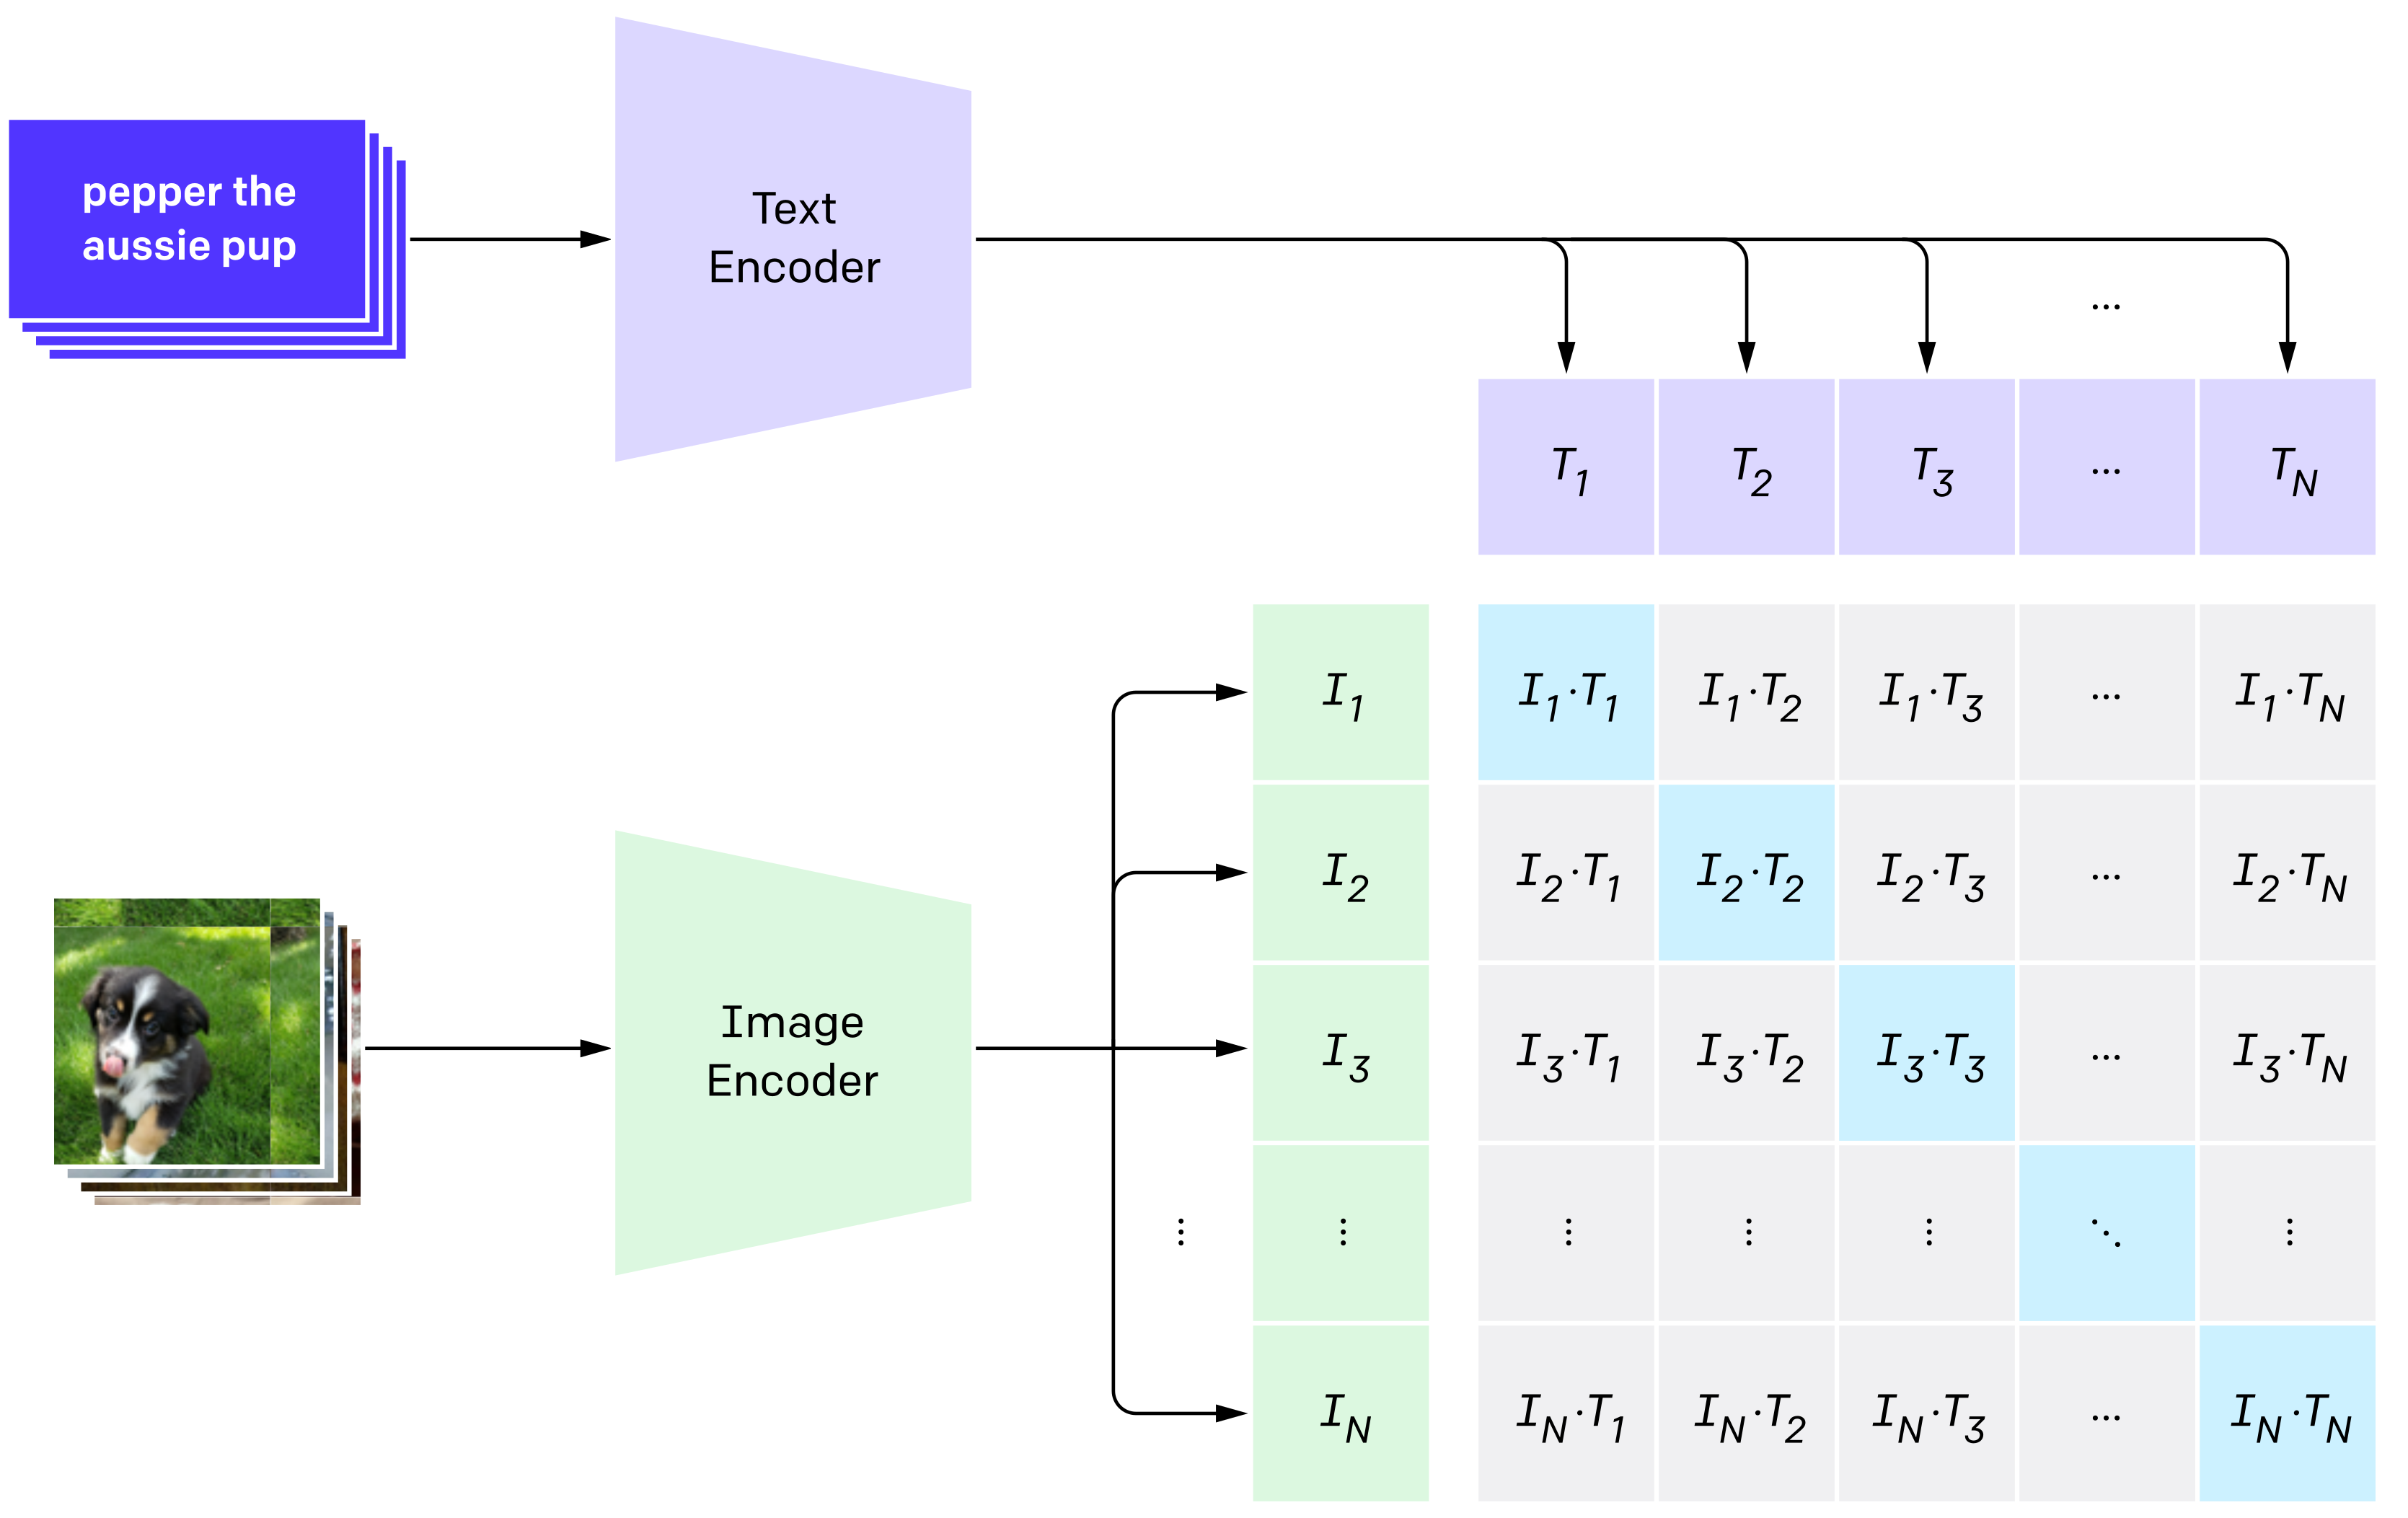
\includegraphics[width=\linewidth, keepaspectratio]{image/clip-a.png}
  \caption{CLIPの事前学習 \cite{clip}}
  \label{fig:clip-a}
\end{figure}
% 
CLIPは対照学習 (Contrastive Learning) と呼ばれる学習手法を採用しており,類似した特徴量間(正例)の類似度は大きく,類似していない特徴量間(負例)の類似度は小さくなるように学習が行われる.
具体的には,$N$個のテキストと画像のペアが入力され,画像エンコーダ (Image Encoder) やテキストエンコーダ (Text Encoder) によって,それぞれの特徴量が埋め込まれる.
$N$枚の画像から得られる特徴量は$I_1, I_2, \ldots, I_N$と,$N$個のテキストから得られる特徴量は$T_1, T_2, \ldots, T_N$と表される.
次に,埋め込まれた特徴量間のコサイン類似度が計算され,正例のコサイン類似度 $I_1 \cdot T_1, I_2 \cdot T_2, \ldots, I_N \cdot T_N$ を最大化し,負例のコサイン類似度を最小化するように画像エンコーダとテキストエンコーダのパラメータを更新する.
この対照学習により,CLIPは画像のみの学習では表現が困難であった,意味的な特徴抽出が可能となる.
また,CLIPは膨大な量の画像とテキストのペアを学習したことにより,タスク固有のデータセットによる追加学習を必要としないZero-Shotタスクに対して高いパフォーマンスを示すことが確認されている.

本研究では,テキストを用いた対照学習によって意味的な特徴表現が可能であるCLIPのIFORに対する有効性を検証する.
ただし,本研究では大規模なテキストと画像による対照学習が行われたCLIPモデルについて,画像エンコーダのみを特徴抽出器として採用する.

\subsection{転移学習}

一般的に,深層学習モデルは大規模なデータセットを用いた学習により高い汎化能力を獲得することが知られている.
一方で,学習用データを十分に確保できない場合,過学習が起こる可能性が高く,モデルが十分な汎化性能を得ることは極めて困難である.
実世界のタスクにおいては,多くの場合,大規模な学習データセットの構築が現実的に困難である.

これらの問題に対して,小規模なデータセットを用いて効率的にモデルの学習を行うFSLタスクでは,転移学習が重要な解決策として知られている.
図 \ref{fig:transfer_image}に転移学習の概要を示す.
% 
\begin{figure}[tbp]
  \centering
  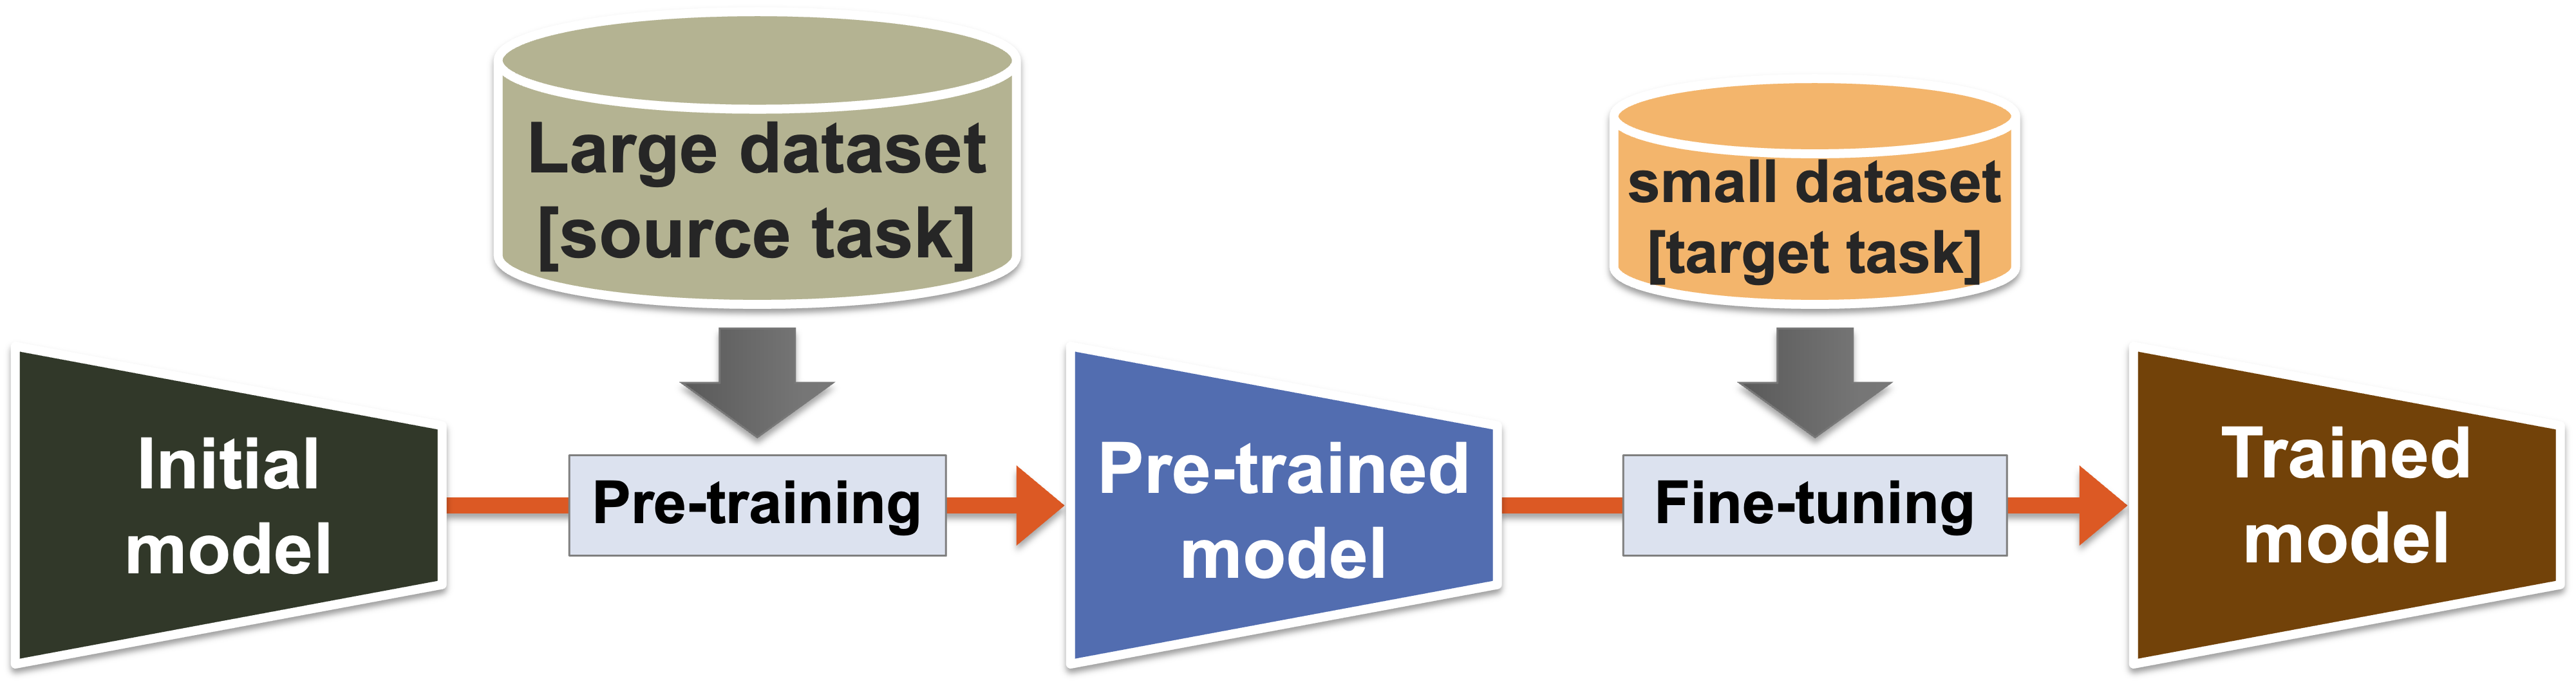
\includegraphics[width=\linewidth, keepaspectratio]{image/transfer_learning.png}
  \caption{転移学習の概要}
  \label{fig:transfer_image}
\end{figure}
% 
転移学習とは,事前に別のタスクから得られた知識を活用し,関連する新しいタスクに対して深層学習モデルの汎化性能を向上させる手法である.
この手法により,広範な学習データから得られた汎用的なモデルの知識を転移させることで,少量の学習データしかない場合においても深層学習モデルは高精度な分類が可能となる.

本研究ではIFORフレームワークにおける転移学習の有効性について検証を行う.
転移学習による性能向上において,事前学習のタスク(ソースタスク)と本番環境でのタスク(ターゲットタスク)の類似性は重要な要素である.
そこで,IFORのターゲットタスクが赤外線画像であることを考慮し,色情報を含まないフラクタル画像を事前学習に用いるFormula-Driven Supervised Learning (FDSL) \cite{fdsl}の適用可能性について評価を行う.
また,事前学習データセットとして様々な画像認識タスクで標準的に用いられており,包括的な画像を含んだ大規模データセットImageNetを用いた事前学習の有効性についても検証を行う.
図 \ref{fig:transfer_learning}に,それぞれのデータセットにおける画像の例を示す.
FDSLでは,数式によって生成されたフラクタル幾何画像を用いており,色情報が含まれないため,形状特徴を強調した特徴抽出器の学習が期待できる.

\begin{figure}[tbp]
  \centering
  \begin{subfigure}[b]{0.45\linewidth}
    \centering
    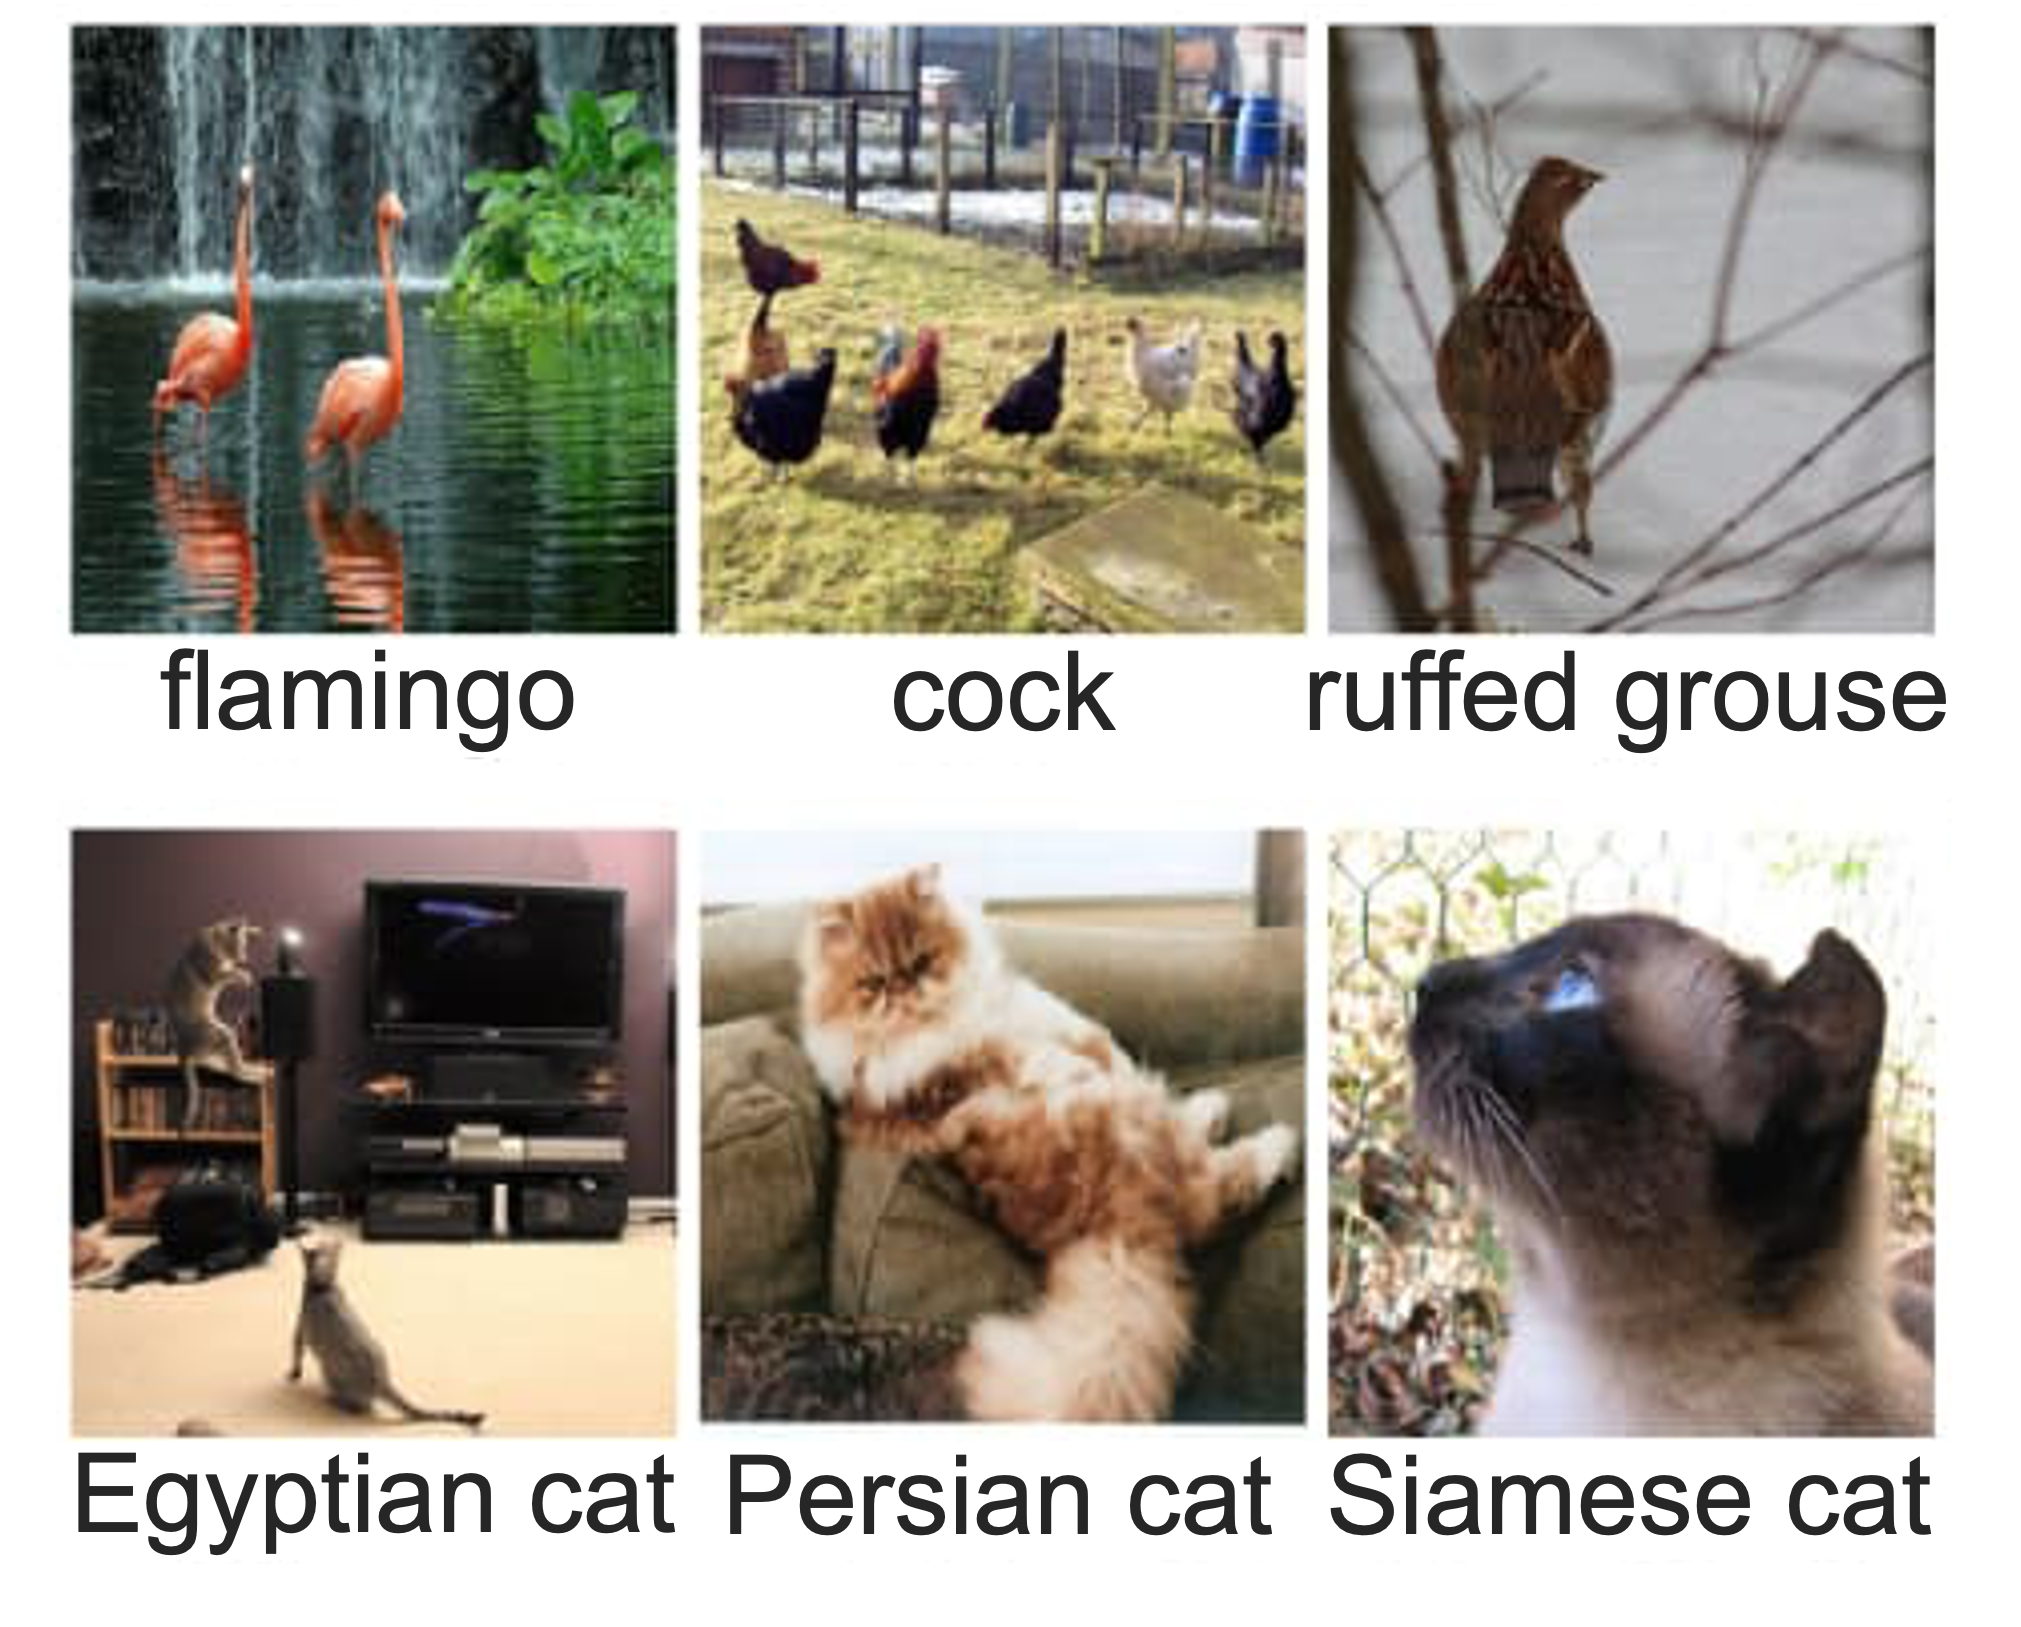
\includegraphics[height=0.9\linewidth, keepaspectratio]{image/imagenet.png}
    \caption{ImageNetの画像例}
    \label{fig:imagenet}
  \end{subfigure}
  \hfill
  \begin{subfigure}[b]{0.45\linewidth}
    \centering
    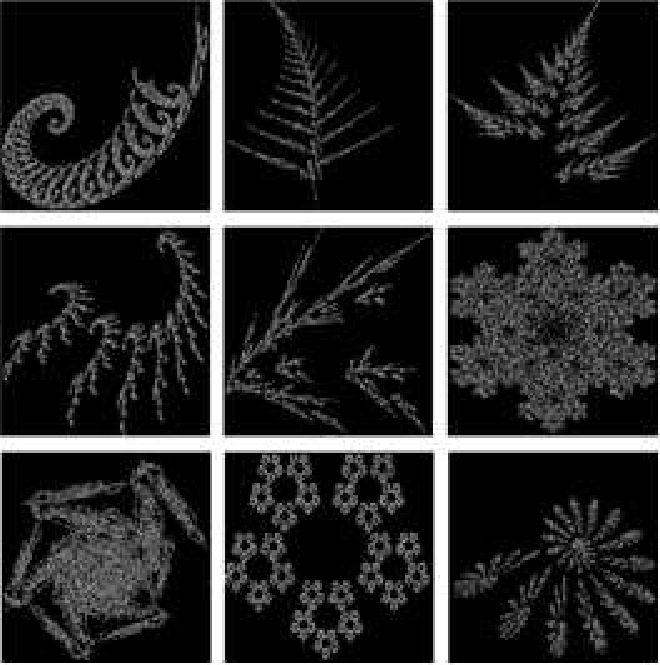
\includegraphics[height=0.9\linewidth, keepaspectratio]{image/fdsl.png}
    \caption{FDSLの画像例}
    \label{fig:fdsl}
  \end{subfigure}
  \caption{ImageNetとFDSLの画像例}
  \label{fig:transfer_learning}
\end{figure}

\subsection{メタ学習}

メタ学習は,学習方法の学習として知られており,FSLにおける効率的なアプローチとして広く認識されている.
図 \ref{fig:meta-learning}にメタ学習の概要図を示す.
% 
\begin{figure}[tbp]
  \centering
  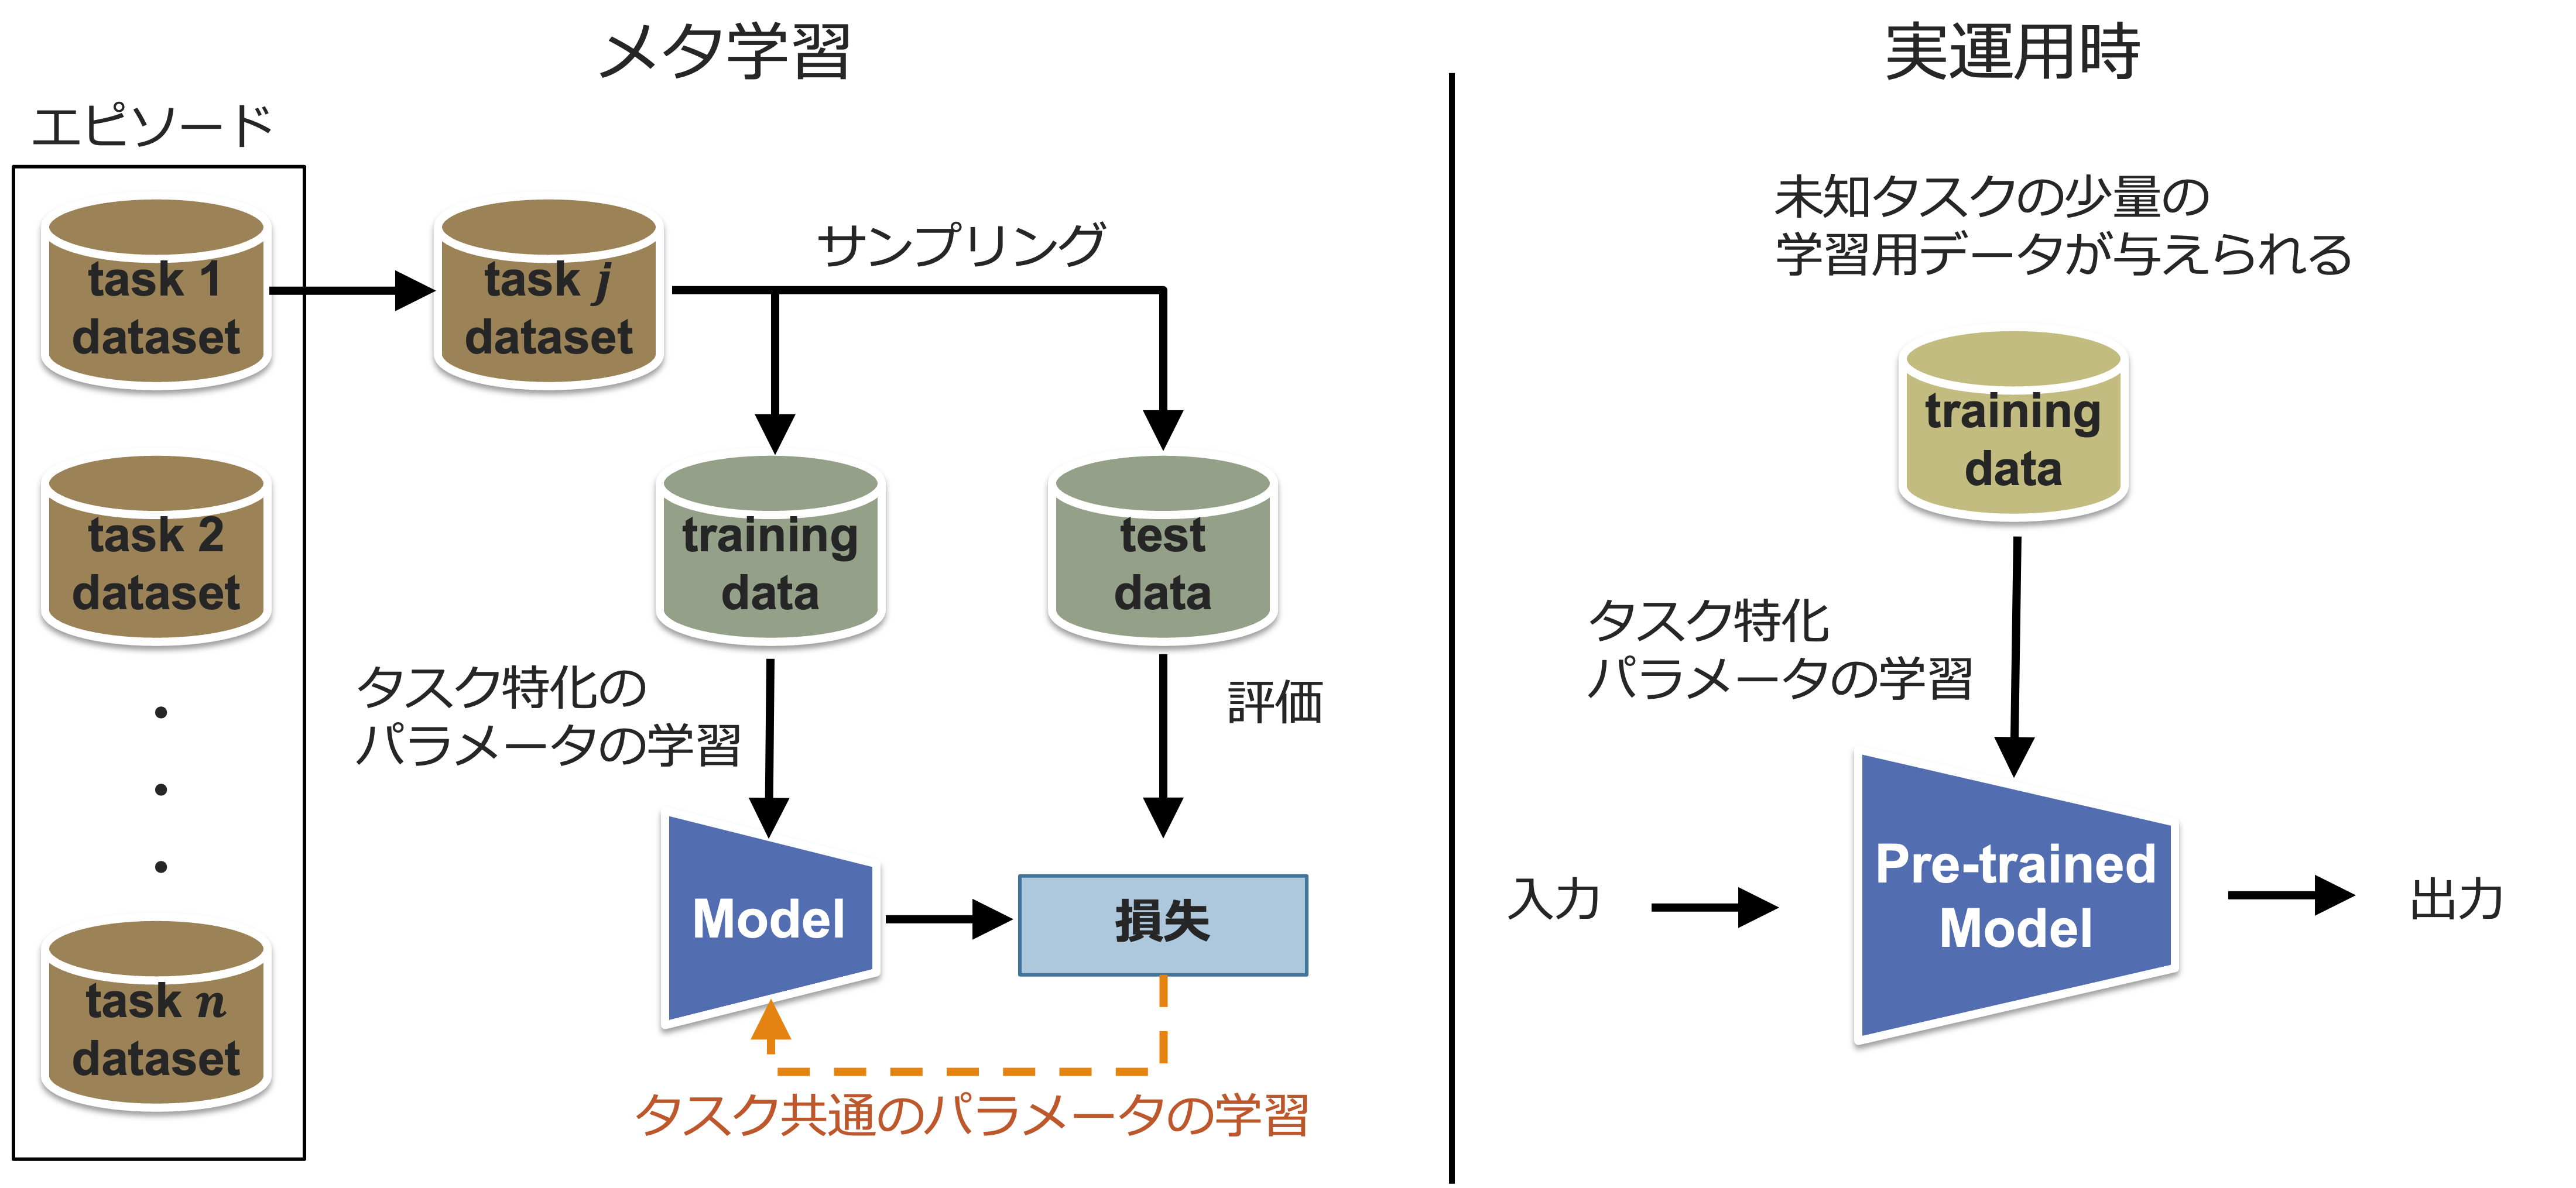
\includegraphics[width=\linewidth, keepaspectratio]{image/meta-learning.png}
  \caption{メタ学習の概要}
  \label{fig:meta-learning}
\end{figure}
% 
メタ学習では,様々なタスクによって構成される学習単位をエピソードと呼び,深層学習モデルは複数のエピソードを通じて学習アルゴリズムを改善し,
限られたデータに対する汎化性能を強化する.
各タスクは,それぞれ$K$個のデータを持つ$N$個のクラスで構成されており,このタスク設定は``$N$-Way, $K$-Shot分類''と呼ばれる.

メタ学習の各エピソードでは,ランダムに選択された学習タスクに基づいてモデルパラメータが更新される.
このプロセスにより,モデルは各エピソードで異なるタスクへの対応を求められ,特定のサブセットではなくより一般的な特徴表現の獲得が期待される.

Snellらは,FSLの代表的なメタ学習手法であるPrototypical Networks (ProtoNet) を提案した \cite{protonet}.
ProtoNetの概要を図 \ref{fig:protonet}に示す.
% 
\begin{figure}[tbp]
  \centering
  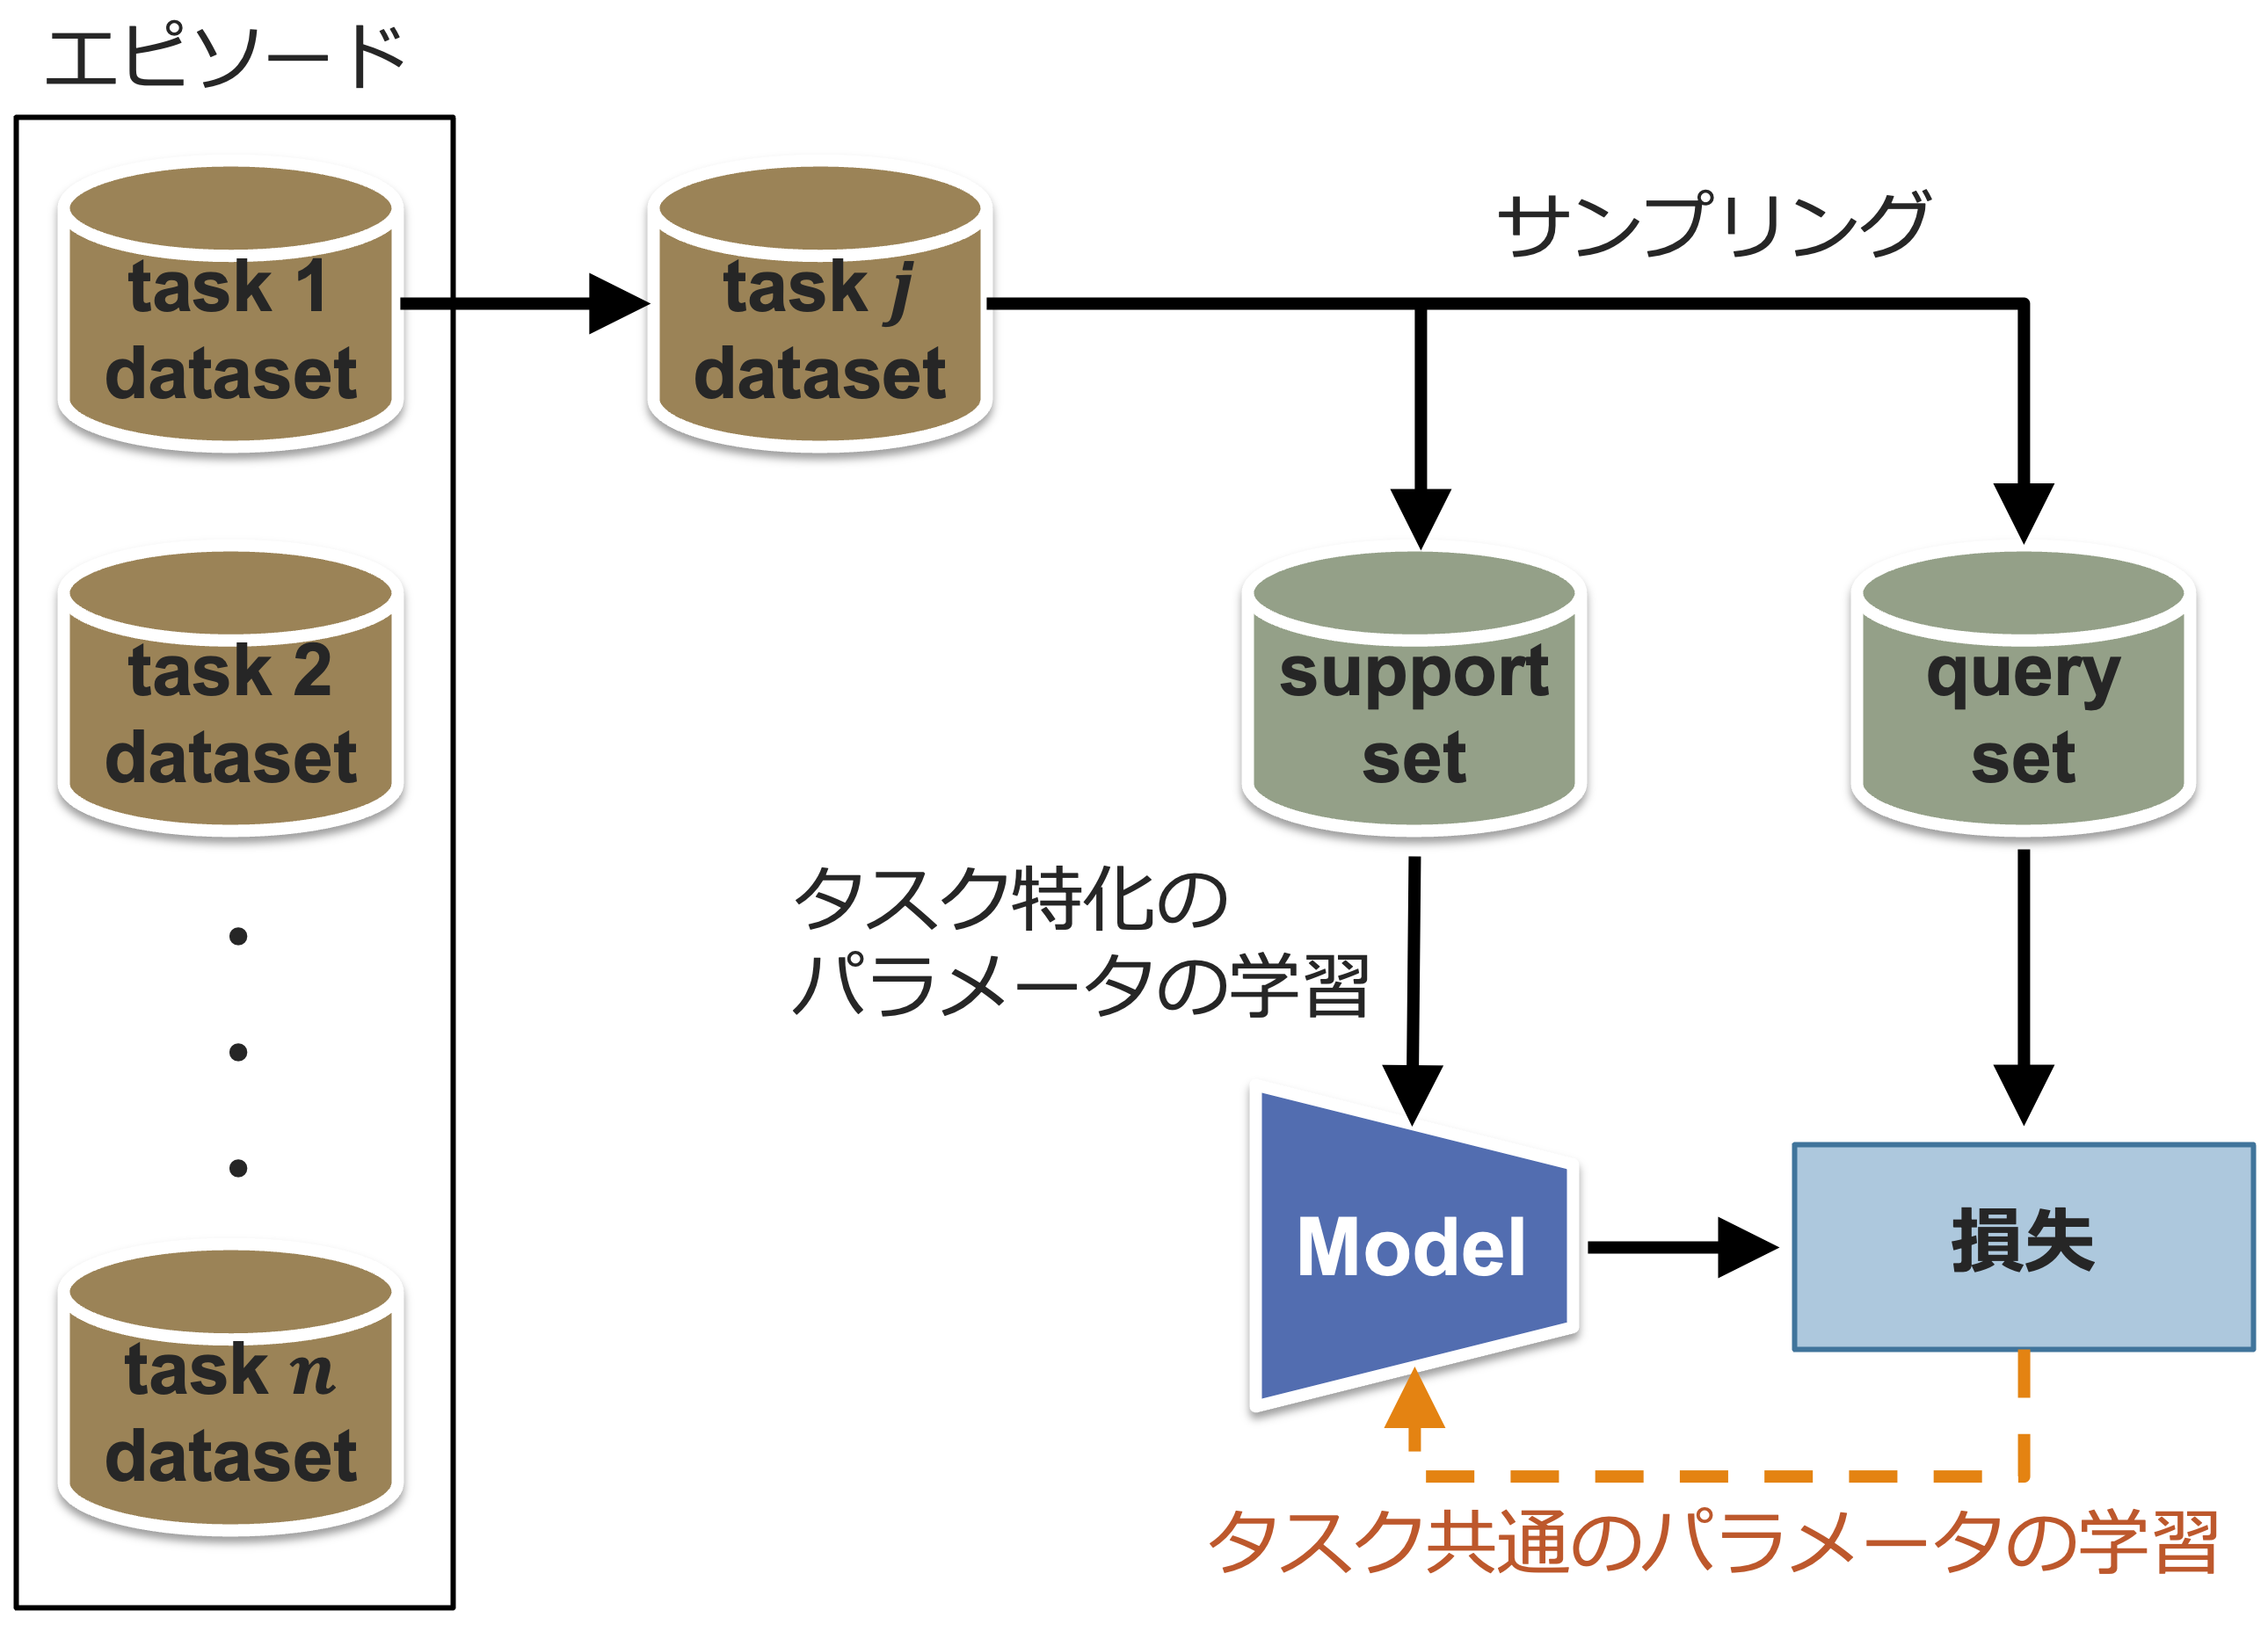
\includegraphics[width=0.7\linewidth, keepaspectratio]{image/protonet.png}
  \caption{ProtoNetの概要}
  \label{fig:protonet}
\end{figure}
% 
ProtoNetでは,モデルに登録するクラスセットであるサポートセット (support-set) と,サポートセットを評価するためのクエリセット (query-set) を用いて学習を行う.
ProtoNetは,入力データと各クラスのプロトタイプとの距離に基づき分類のための特徴空間を学習することにより,少数データにおける分類を実現する.
プロトタイプはサポートセットの埋め込みベクトルの平均として定義される.
具体的に,サポートデータは各クラスのプロトタイプを中心としたクラスタを形成するような空間に埋め込まれ,
分類時には,クエリデータの埋め込みベクトルに最も近いプロトタイプを持つクラスが予測クラスとして分類される.
このような距離に基づく分類手法により,FSLにおいて課題となる過学習に対処している.

近年,メタ学習アルゴリズムがFew-Shot Open-Set Recognition (FSOSR) の分野に拡張され,
登録クラスの分類と未登録クラスの検出の両方を同時に高い精度で実現する手法が提案された.
Liuらは,モデルの学習過程で登録クラスの分類と未登録クラスの検出に取り組むPEELERアルゴリズムを提案した \cite{peeler}.
従来のソフトマックス分類器は,学習クラスを過剰に適合させる傾向があるため,未登録クラスの検出が困難であった.
PEELERはこの課題に対し,エピソードごとに新規クラスをランダムに選択し,これらのクラスの事後エントロピーを最大化することにより未登録クラスの検出能力の向上を図っている.
さらに,メタ学習をオープンセット認識に拡張したことにより,より一般化された特徴抽出における表現力を獲得し,
認識タスクの様々なスケールや複雑さに対して効果的な学習フレームワークを提供する.

PELLERの概要を図 \ref{fig:peeler}に示す.
% 
\begin{figure}[tbp]
  \centering
  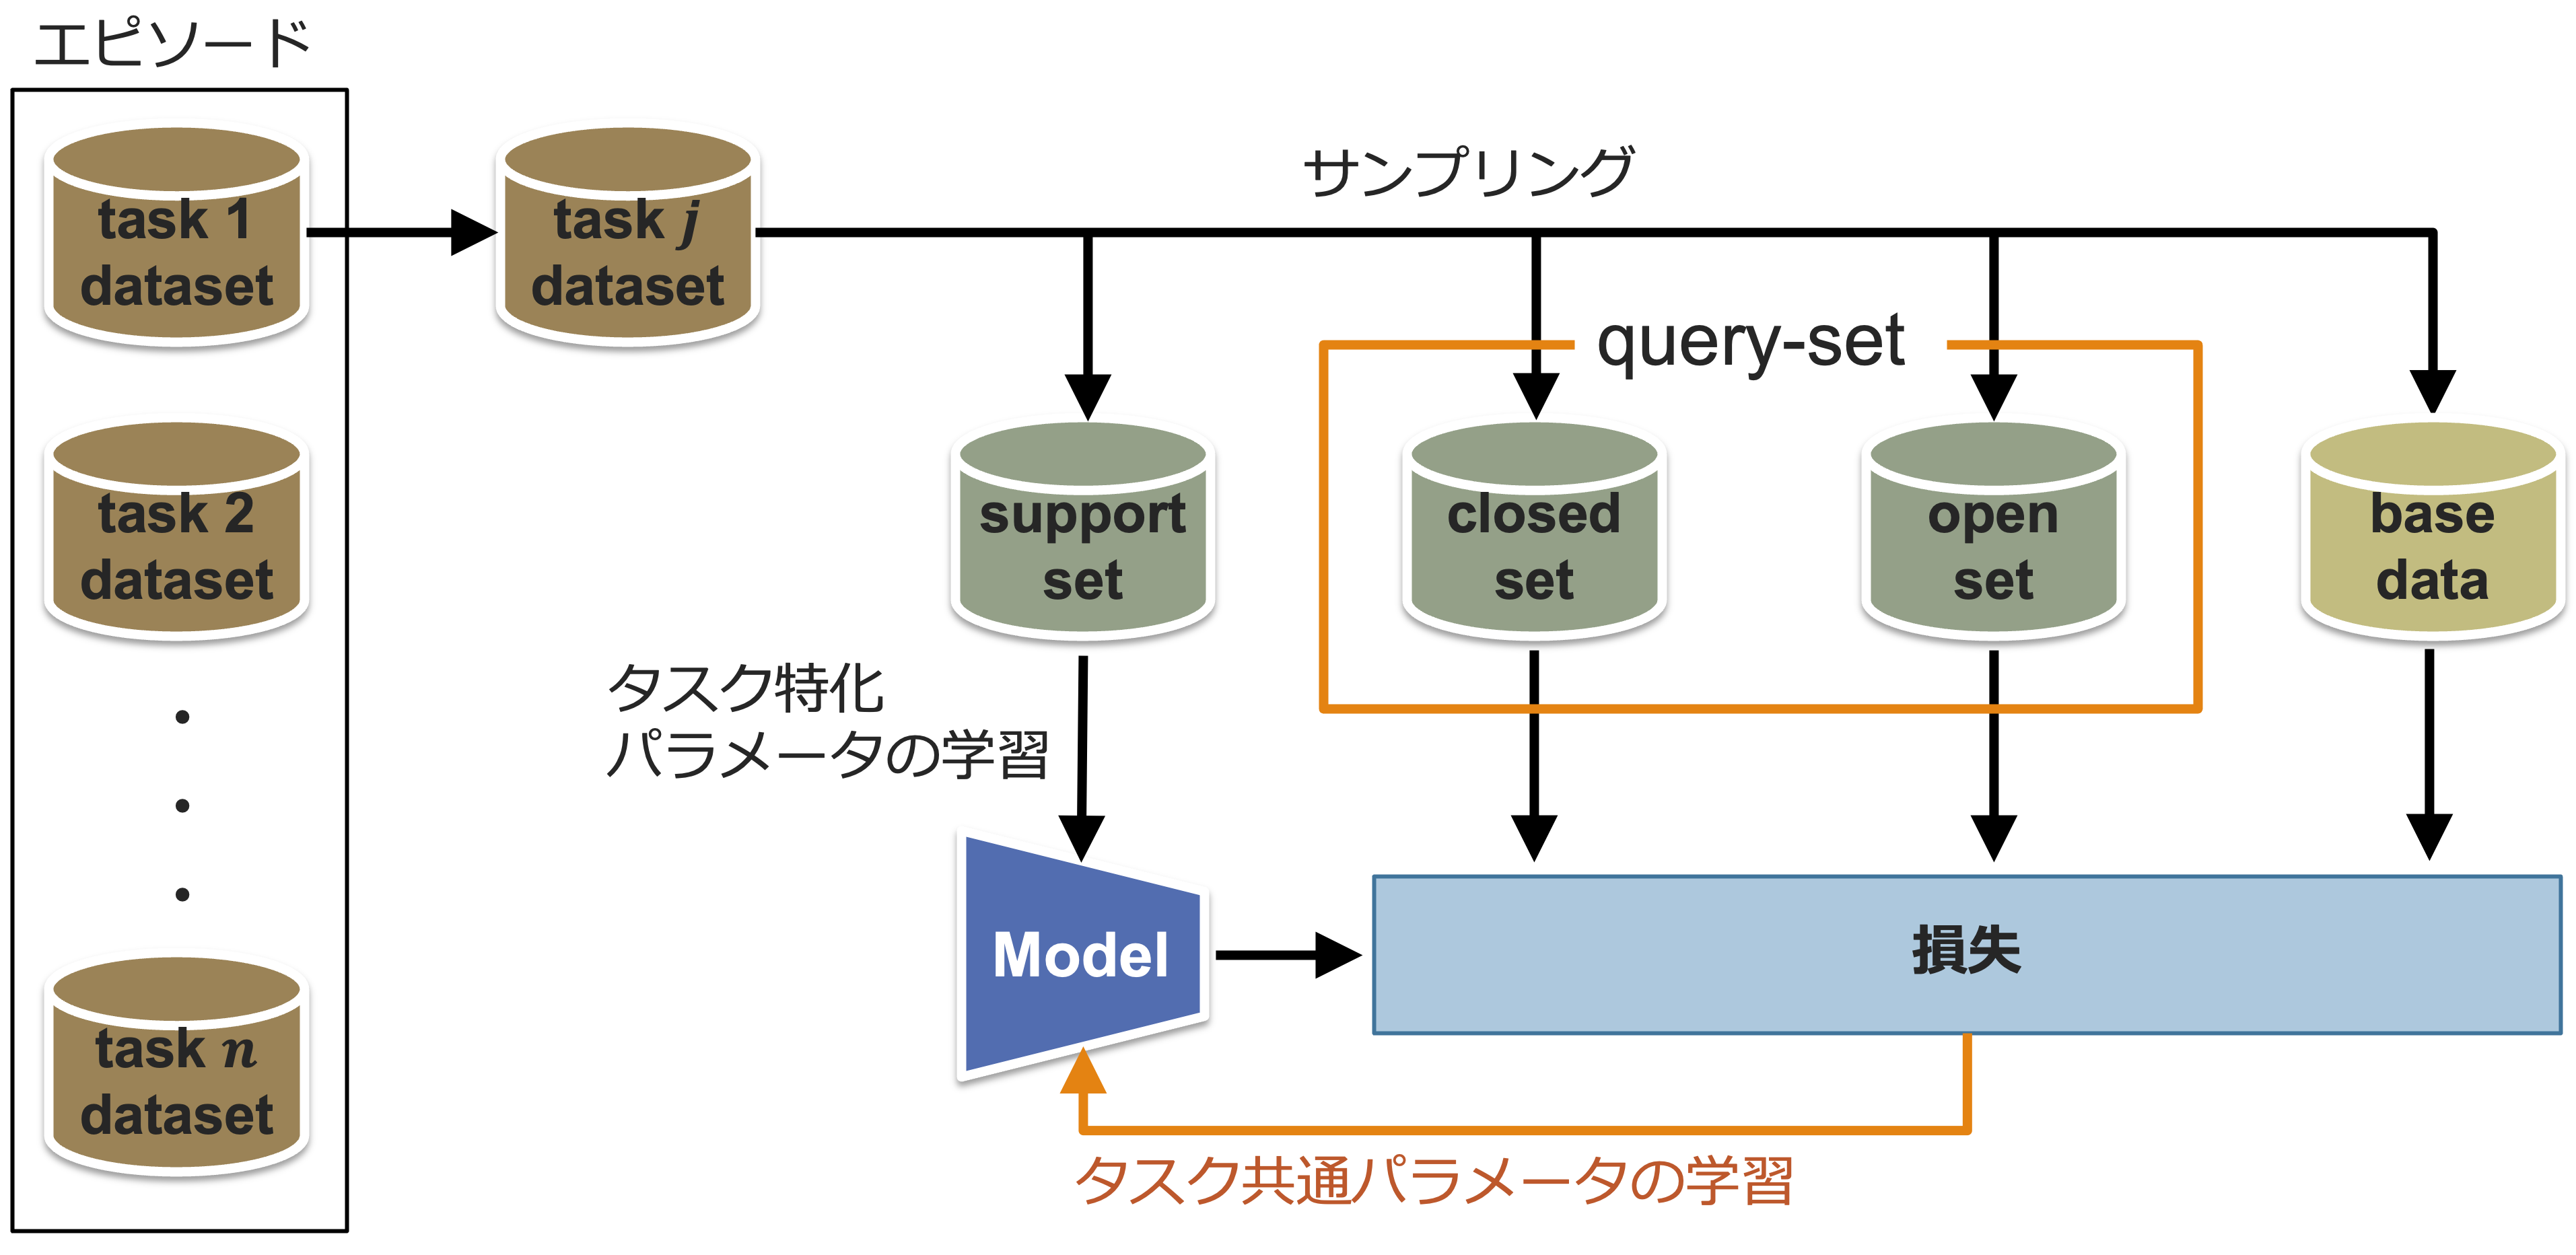
\includegraphics[width=\linewidth, keepaspectratio]{image/peeler.png}
  \caption{PEELERの概要}
  \label{fig:peeler}
\end{figure}
% 
各タスクではサポートセット (support-set) と呼ばれる登録用データとクエリセット (query-set) と呼ばれる評価用データを使用する.
$N$-Way, $K$-Shot分類におけるサポートセットは$\mathcal{D}^S = \left\{ \bm{x}^S_i, y^S_i \right\}^{NK}_{i=1}$と表される.
ここで,$\bm{x}^S_i \in \mathcal{X}^S$はサポートセットの入力画像空間$\mathcal{X}^S$における入力画像であり,$y^S_i \in \mathcal{Y}^S$は登録クラス空間$\mathcal{Y}^S$における教師ラベルを示す.
また,$N$はサポートセットのクラス数,$K$は各クラスのサンプル数を表す.
さらに,クエリセットはサポートセットと同じクラスから構成されるクローズドクエリセット (closed-query set) と,
サポートセットと異なるクラスから構築されるオープンクエリセット (open-query set) の2つに分けられる.
クローズドクエリセットは$\mathcal{D}^C = \left\{ \bm{x}^C_i \in \mathcal{X}^C, y^C_i \in \mathcal{Y}^S \right\}^{NQ}_{i=1}$と表される.
ここで,$\bm{x}^C_i$はクローズドクエリセットの入力画像空間$\mathcal{X}^C$における入力画像であり,$y^C_i$は登録クラス空間$\mathcal{Y}^S$における教師ラベルを示す.
また,$N$はクローズドクエリセットのクラス数,$Q$は各クラスのサンプル数を表す.
一方で,オープンクエリセットは$\mathcal{D}^O = \left\{ \bm{x}^O_i \in \mathcal{X}^O, y^O_i \in \mathcal{Y}^O \right\}^{N^U}_{i=1}$と表される.
ここで,$\bm{x}^O_i$はオープンクエリセットの入力画像空間$\mathcal{X}^O$における入力画像であり,$y^O_i$は未登録クラス空間$\mathcal{Y}^O$における教師ラベルを示す.
また,オープンクエリセットはモデルに未登録のデータ集合であるため$\mathcal{Y}^S \cap \mathcal{Y}^O = \emptyset$ が成り立つ.
サポートセットやクローズドクエリセットがクラス数を明示的に定義するのに対し,オープンクエリセットは未登録クラスの検出を目的とするため,クラス数を定義せず総サンプル数$N^U$のみで表される.
PEELERではこの未登録クラスを単一クラスとして定義することにより,未登録クラスの検出に焦点を当てている.
サポートデータ,クローズドクエリデータ,オープンクエリデータの選択方法の概要を図 \ref{fig:peeler_data}に示している.
% 
\begin{figure}[tbp]
  \centering
  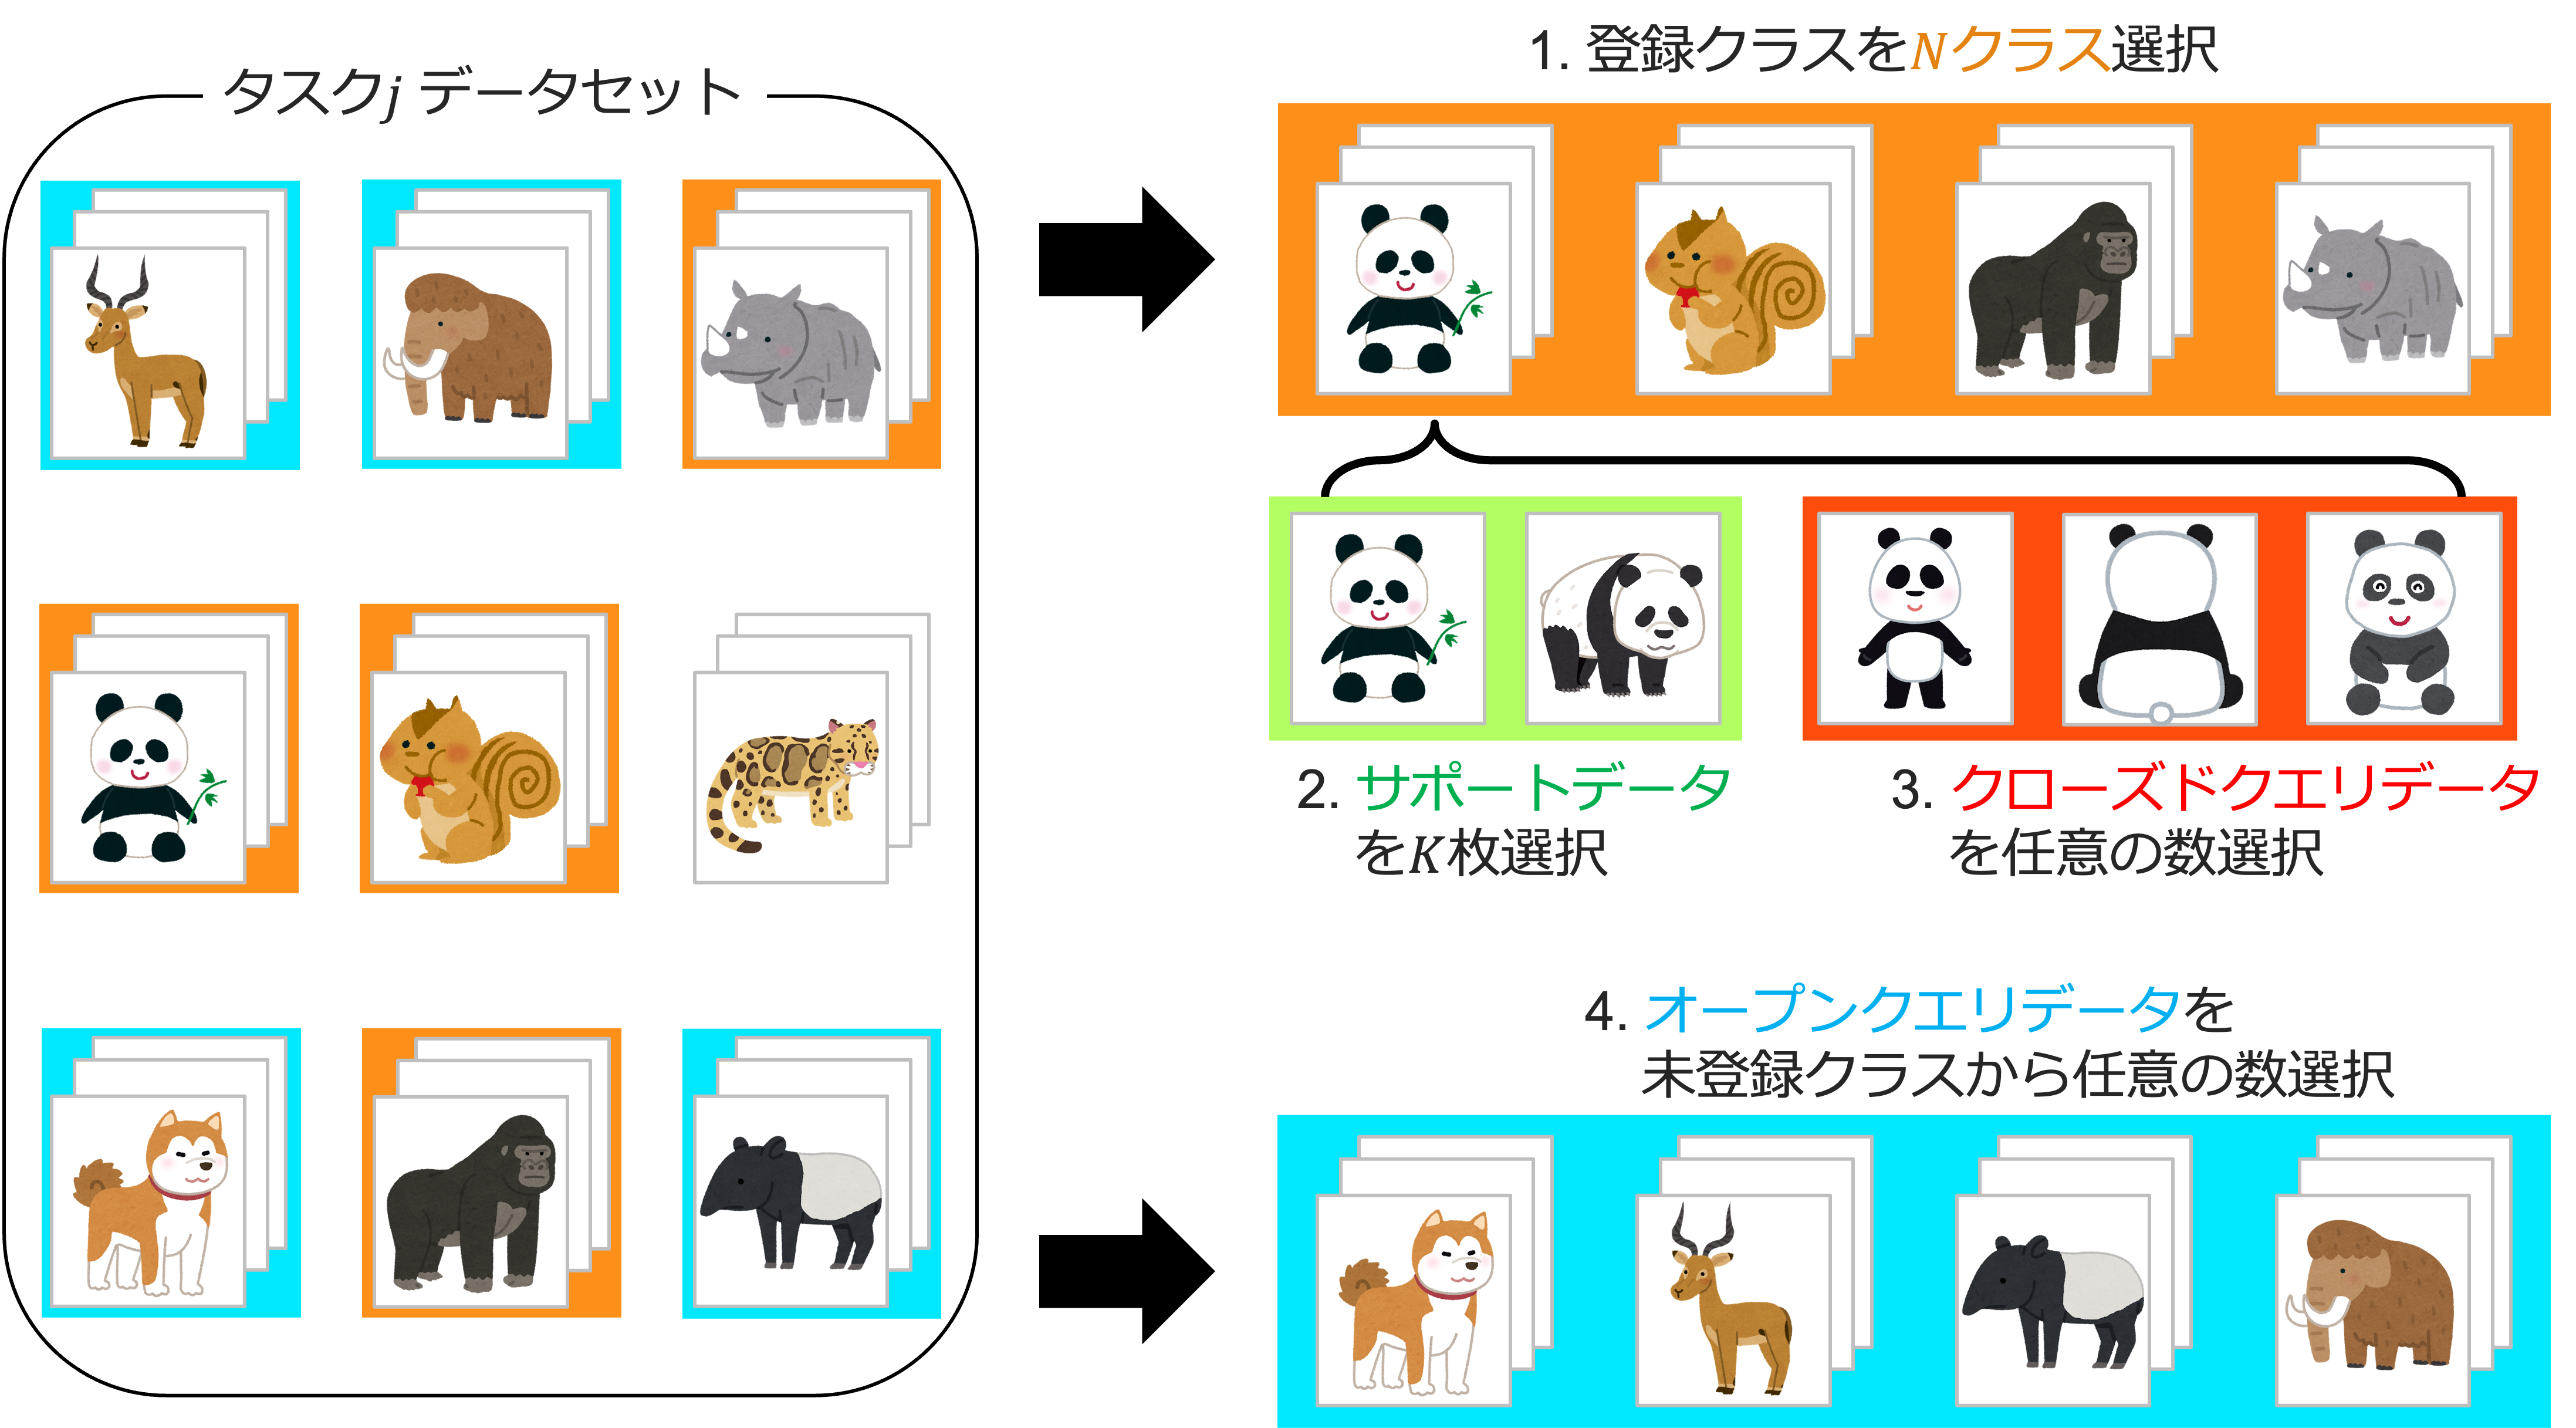
\includegraphics[width=\linewidth, keepaspectratio]{image/meta-class.png}
  \caption{登録クラス・未登録クラスの選択方法}
  \label{fig:peeler_data}
\end{figure}
%
PEELERは,プロトタイプと入力データとの距離に基づいて分類を行う.
具体的には,クエリデータが各プロトタイプの閾値より大きい場合は未登録クラス,閾値よりも小さい場合は最も近いプロトタイプのクラスに分類される.
PEELERはモデルに登録されたクラスの分類と未登録クラスの検出において高い精度を達成するため,FSL損失,OSR損失,分類損失の3つの異なる損失関数を採用している.
FSL損失は,プロトタイプとクローズドクエリセットを近づけることで,少数データにおける登録クラスの分類性能を向上させる.
OSR損失はプロトタイプとオープンクエリセットを離すことで,未登録クラスの検出精度を向上させる.
最後に,分類損失は,ランダムな画像から構成されるベースデータから適切な特徴を抽出し,モデルの分類能力を最適化するように設計されている.
エピソードを通してタスク間で異なるクラスセットを学習することにより,モデルは特定のタスクではなく,タスク間の共通性を学習することが期待される.

FSL損失の導出には,学習用データセットから選択されるサポートセットとクローズドクエリセットが用いられる.
メタ学習の過程において,クローズドクエリデータから抽出された特徴ベクトルをサポートデータの正解クラスに近づける学習を行うことで,
モデルは正確な分類を実現する特徴マッピングが習得可能となる.
図\ref{fig:fsl_loss}では,FSL損失で学習することにより効果的に登録クラスの分類が可能になる例を示している.
% 
\begin{figure}[tbp]
  \centering
  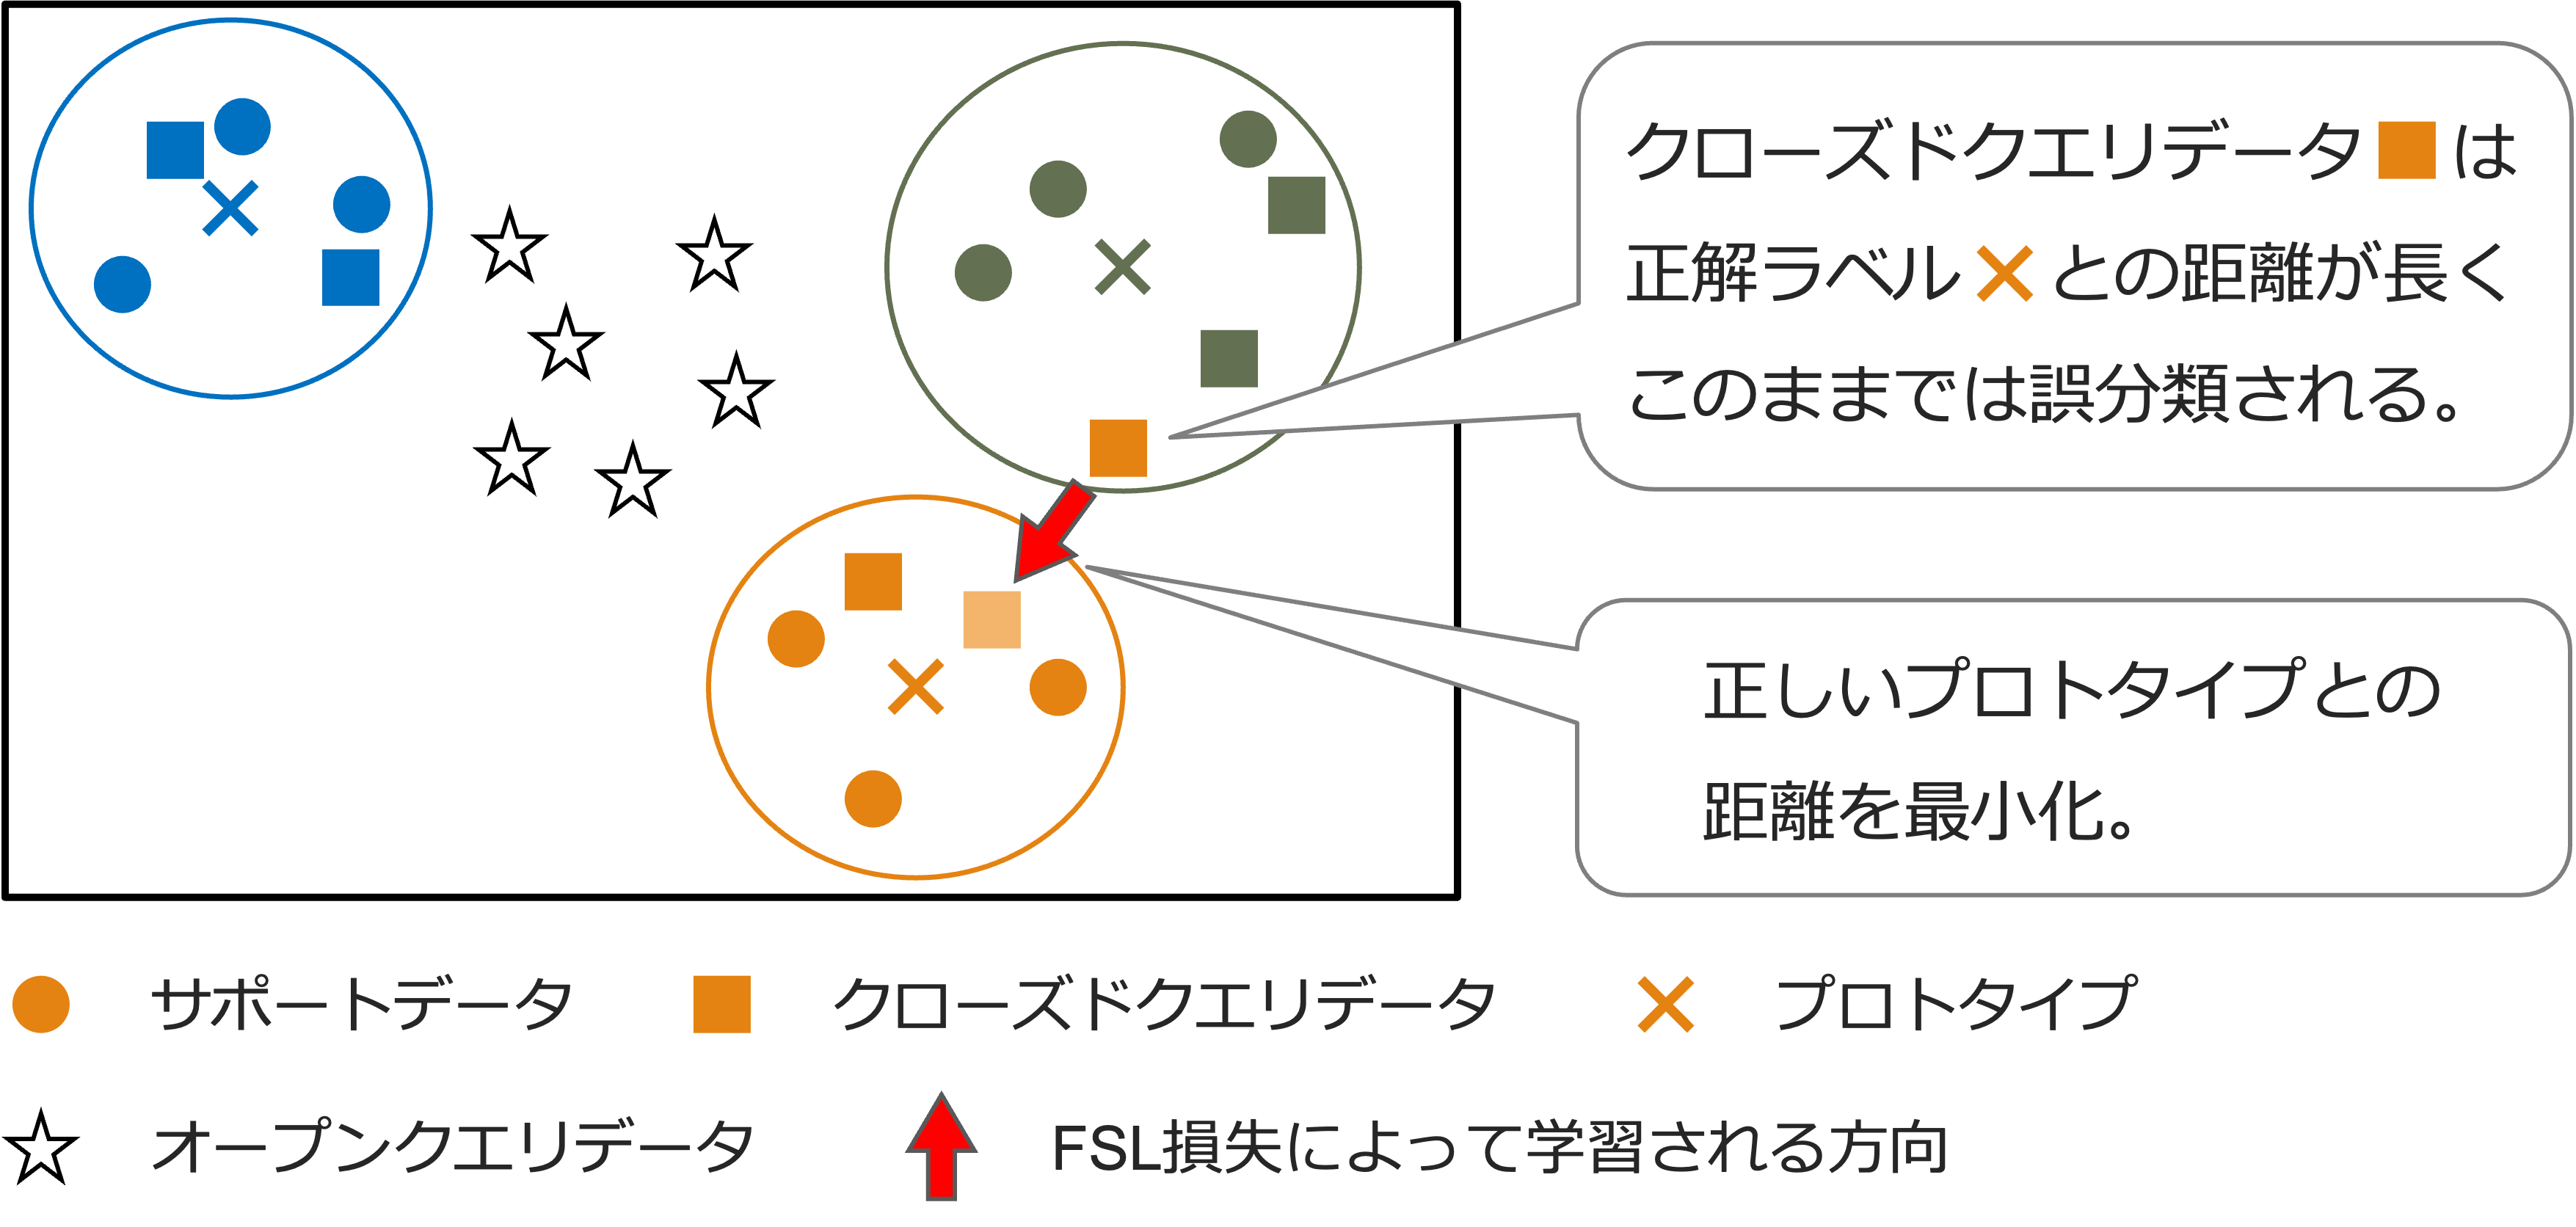
\includegraphics[width=\linewidth, keepaspectratio]{image/fsl_loss.png}
  \caption{FSL損失での学習が登録クラスの分類精度を向上させる例}
  \label{fig:fsl_loss}
\end{figure}
% 
以下に具体的なFSL損失の導出過程を述べる.

まず,プロトタイプとクローズドクエリデータの特徴ベクトル間のユークリッド距離を計算する.

\begin{equation}
  dist(f_{\phi}(\bm{x^C}),\mu_{k})=(f_{\phi}(\bm{x^C}) - \mu_{k})^{\top} (f_{\phi}(\bm{x^C}) - \mu_{k})
\end{equation}

\noindent
ここで,$f_{\phi}(\bm{x^C}) \in \mathcal{F}$ はクローズドクエリセットにおける入力画像 $\bm{x}^C \in \mathcal{X}^C$ の特徴ベクトルを表す.
ただし,$\mathcal{X} \subseteq \mathbb{R}^D$ は$D$次元の入力画像空間, $\mathcal{F} \subseteq \mathbb{R}^V$ は$V$次元の特徴空間を表す.
また,$f_{\phi}: \mathcal{X} \rightarrow \mathcal{F}$ はニューラルネットワークによる特徴抽出器であり,$\phi$ は学習可能なパラメータである.
$\mu_{k}$ は$k$番目のクラスのプロトタイプを表し,以下の式で算出される.

\begin{equation}
  \mu_{k} = \frac{1}{K} \sum_{\bm{x}^S_i \in \mathcal{X}^S_k} {f_\phi(\bm{x}^S_i)}
\end{equation}

\noindent
ここで,$\mathcal{X}^S_k$はクラス$k$におけるサポートデータ集合である.

次に,ユークリッド距離に負の符号を付けてソフトマックス関数に適用する.

\begin{equation}
\label{eq:fsl_prob}
  p_{\phi}(y^C=k \mid \bm{x}^C, \mathrm{M}) 
              = \frac{\exp(-dist(f_\phi(\bm{x}^C),\mu_{k}))}{\sum_{i \in \mathcal{Y}^S} {\exp(-dist(f_\phi(\bm{x}^C),\mu_{i}))}}
\end{equation}

\noindent
ここで,$p_{\phi}(\cdot \mid \cdot, \cdot)$は分類確率を表し,$\mathrm{M} = \left\{\mu_0, \mu_1, \ldots, \mu_{N-1} \right\}$はプロトタイプ集合を示す.
式 \ref{eq:fsl_prob}より,サポートデータとクローズドクエリデータの特徴ベクトル間のユークリッド距離が短いほど,正しく分類できる確率が高くなることが分かる.
よって,深層学習モデルの学習において,プロトタイプとクローズドクエリデータ間の距離が長い場合に大きな損失を与えることが望ましい.
最終的に,FSL損失はクロスエントロピー損失を用いて以下のように計算される.

\begin{equation}
  \mathcal{L}_{\mathrm{FSL}} [y^C, \bm{x}^C] = \sum_{(\bm{x}^C_i,y^C_i) \in \mathcal{D}^C} - \log {p_{\phi} (y^C_i \mid \bm{x}^C_i, \mathrm{M})}
\end{equation}

次に,OSR損失の計算の際は,学習用データセットから選択されるサポートセットとオープンクエリセットが用いられる.
ここで用いるサポートセットとは,前述したFSL損失の計算時に利用したものと同一のサンプルセットである.
一方,オープンクエリセットは,未登録クラスの検出能力を評価するためのサンプルセットであり,学習用データセットからサポートセットと異なるクラスの画像がランダムに選択される.

メタ学習の過程において,オープンクエリデータから抽出された特徴ベクトルを全てのプロトタイプから遠ざけることにより,
深層学習モデルは正確な未登録の検出能力を習得することが期待される.
図 \ref{fig:osr_loss}に,OSR損失で学習することにより効果的に未登録クラスの検出が可能になる例を示す.
% 
\begin{figure}[tbp]
  \centering
  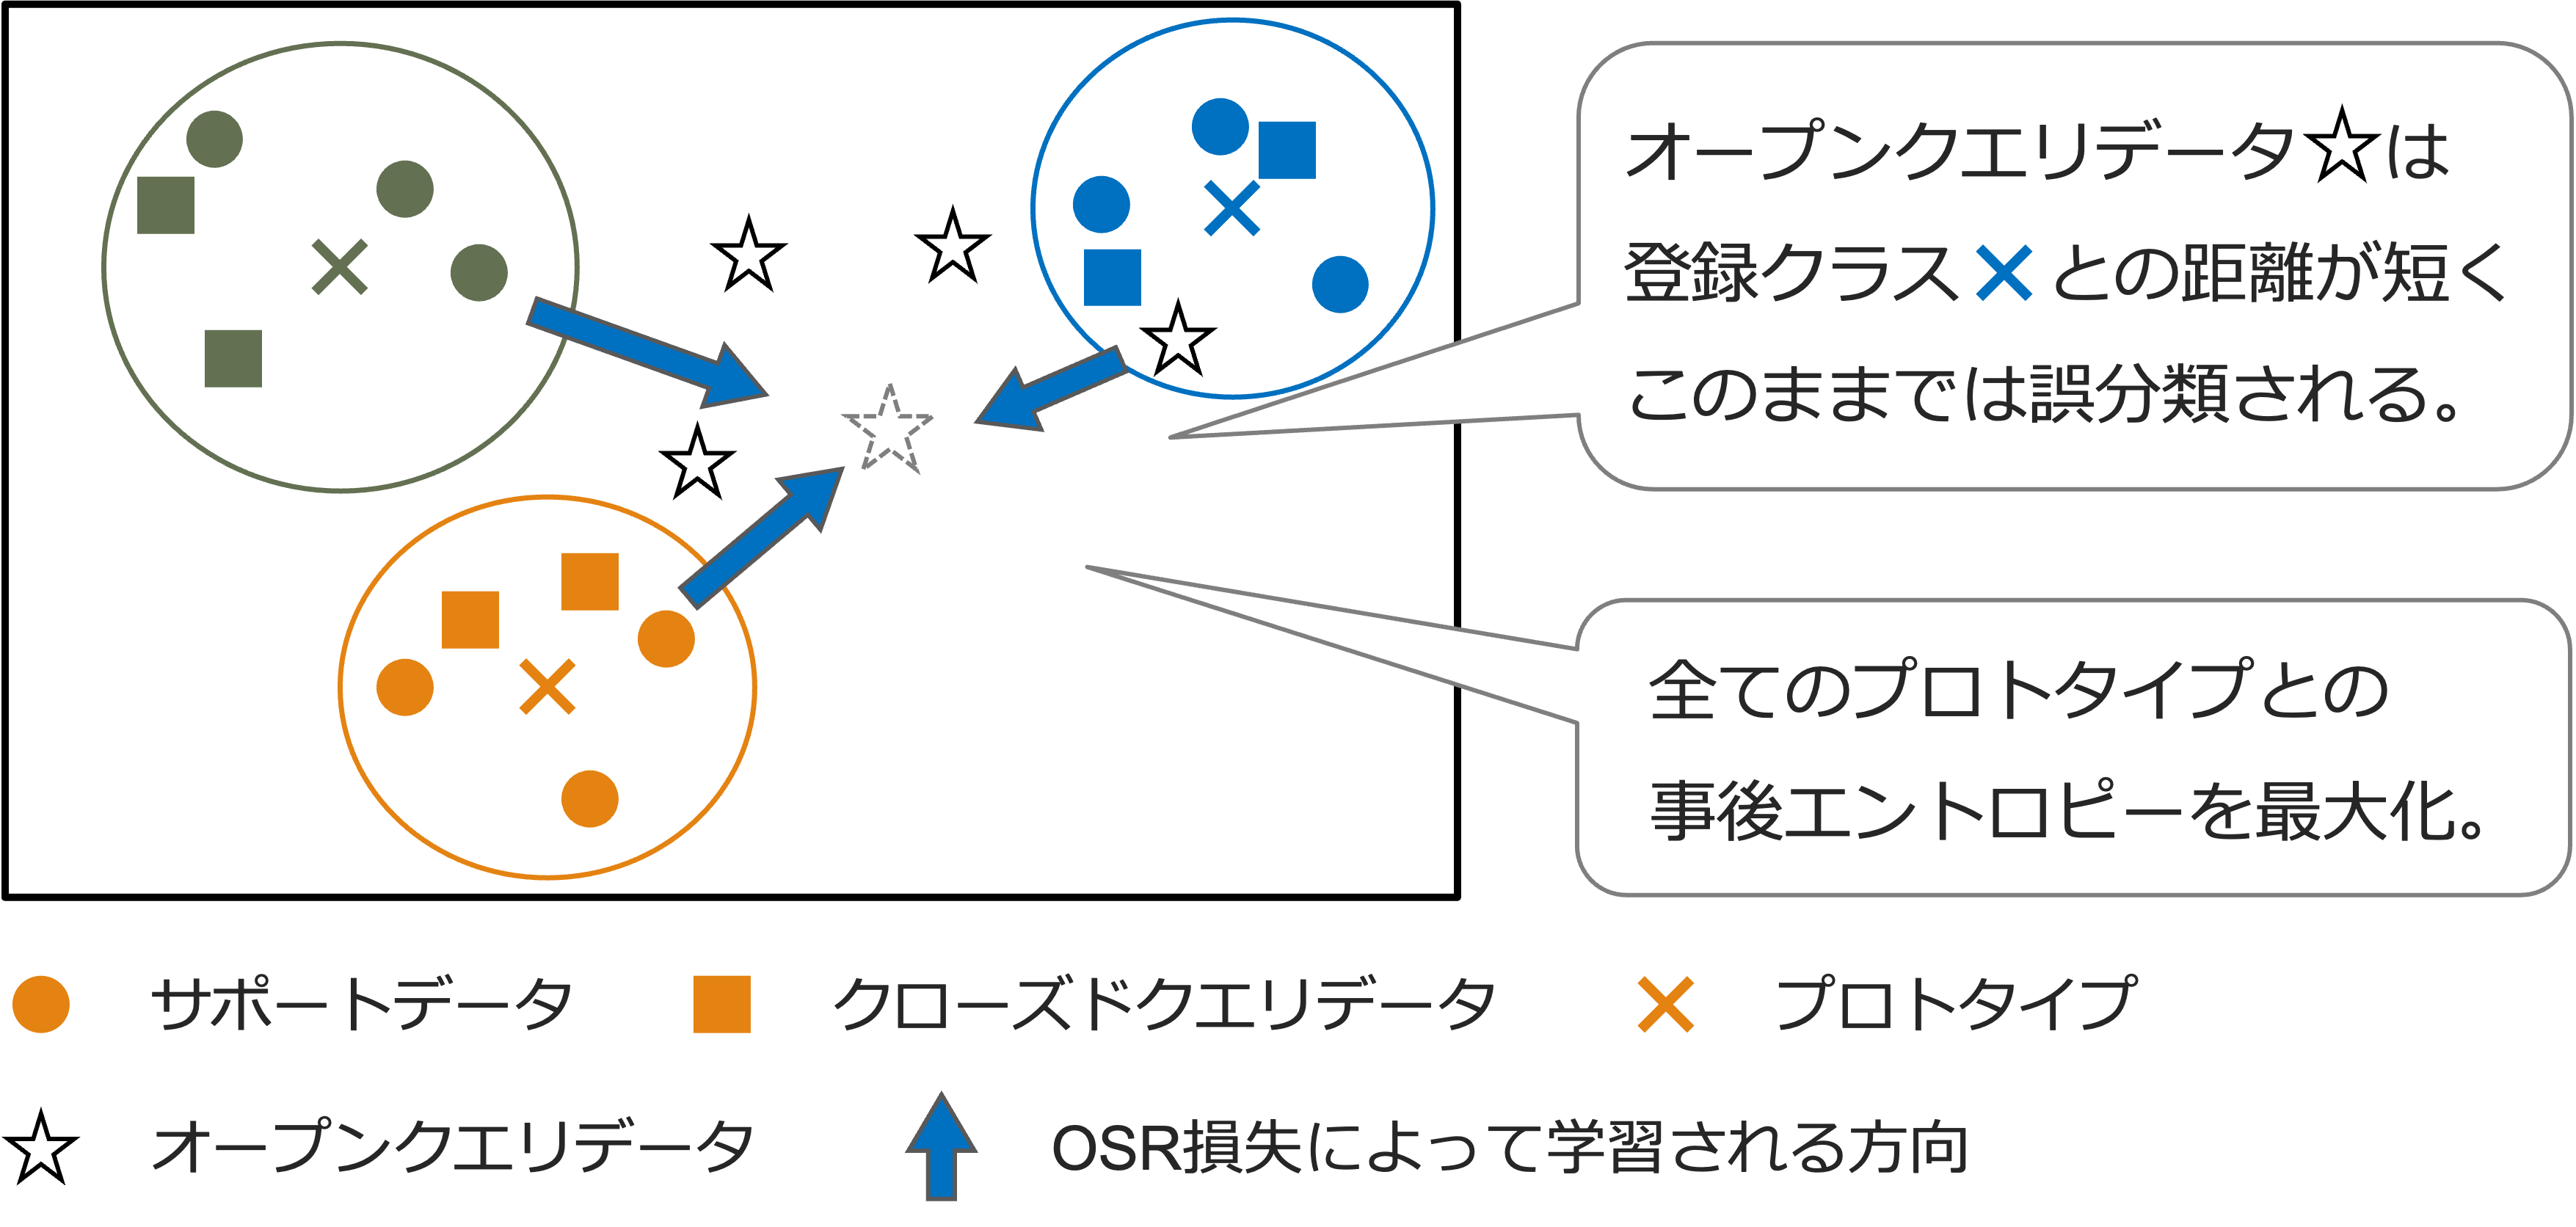
\includegraphics[width=\linewidth, keepaspectratio]{image/osr_loss.png}
  \caption{OSR損失での学習が未登録クラスの検出精度を向上させる例}
  \label{fig:osr_loss}
\end{figure}
% 
以下に具体的なOSR損失の導出過程を述べる.

モデルは,正しく未登録の検出を行うために,未登録クラスからのサンプルに遭遇した際,サポートデータのどのクラスにおいても大きな確率を割り当てるべきではない.
この場合,プロトタイプ集合に対するオープンクエリセットの最大のクラス確率$\underset{k \in \mathcal{Y}^S}{\max} {p_{\phi}(k|\bm{x}^O, \mathrm{M})}$が小さければ,未登録クラスのサンプルを適切に棄却することができる.
この目的を達成するため,PEELERアルゴリズムでは,オープンクエリセットのサンプルに対して,登録済みクラスへの分類確率の最小化を図る.
これは,オープンクエリデータの事後エントロピーを最大化すること,すなわち負のエントロピーを用いることで実現可能である.
この最適化を実現するための損失関数として,OSR損失は以下のように計算される.

\begin{equation}
    \mathcal{L}_{\mathrm{OSR}}[\bm{x}^O]
                = \sum_{k \in \mathcal{Y}^S} {p_{\phi}(k \mid \bm{x}^O, \mathrm{M}) \log{p_{\phi}(k \mid \bm{x}^O, \mathrm{M})}}
\end{equation}

最後に,分類損失の導出では,タスク$j$データセットから任意の数の画像枚数がベースデータとして選択される.
ベースデータは$\mathcal{D}^B = \left\{ \bm{x}^B_i \in \mathcal{X}^B, y^B_i \in \mathcal{Y}^B \right\}^{I J}_{i=1}$と表される.
ここで,$\bm{x}^B_i$はベースデータの入力画像空間$\mathcal{X}^B$における入力画像であり,$y^B_i$は教師ラベル空間$\mathcal{Y}^B$における教師ラベルを示す.
また,$I$はベースデータのクラス数,$J$は各クラスのサンプル数を表す.
% ここで,$\mathcal{X}^B$,$\mathcal{Y}^B$はそれぞれベースデータにおける入力画像空間,教師ラベル空間であり,
% $I$,$J$はそれぞれベースデータのクラス数,下クラスのサンプル数を示す.
この分類損失は,モデルが新しいドメインにおける分類タスクに対して,一般的かつ有用な特徴抽出を学習するために使用される.
モデルは,ベースデータから特徴抽出を行う際は特徴空間上での距離による分類ではなく,分類ヘッドを用いて学習を進める.
これは,学習用データセットに含まれる全てのクラスの分類問題を解くことと同義である.
分類確率の計算は,以下のソフトマックス関数を用いて行われる.

\begin{equation}
    p(y^B=k \mid \bm{x}^B;\phi,\mathbf{w}_k) 
        = \frac{\exp(\mathbf{w}_k^{\top} f_{\phi}(\bm{x}^B))}{\sum_{i \in \mathcal{Y}^B} \exp(\mathbf{w}_{i}^{\top} f_{\phi}(\bm{x}^B))}
\end{equation}

\noindent
ここで,$\mathbf{w}_k$は特徴抽出器の重みベクトルを表す.
よって,分類損失はクロスエントロピー損失を用いて以下のように表される.

\begin{equation}
  \mathcal{L}_{\mathrm{base}} [y^B, \bm{x}^B] = \sum_{(\bm{x}^B_i,y^B_i) \in \mathcal{D}^B} - \log {p(y^B_i \mid \bm{x}^B_i)}
\end{equation}

最終的に,FSL損失,OSR損失及び分類損失を線型結合し,バックプロパゲーションすることによりモデルのパラメータを更新する.
この学習手法により,深層学習モデルは登録クラスの正確な分類と未登録クラスの検出の両方を効果的に実現することが可能となる.
具体的には以下の最適化問題を解くことにより,$e \in \{1, 2, \ldots, N_e\}$エピソードにおけるモデル$h^*$を更新する.

\begin{align}
  h^* & = \arg \min_h \left\{ \sum_{(x_i,y_i) \in \mathcal{D}^C|y_i \in \mathcal{Y}^S}{\mathcal{L}_{\mathrm{FSL}}[y_i,h'(x_i)]} \right. \nonumber \\
      & \hspace{20mm} + \lambda \sum_{(x_i,y_i) \in \mathcal{D}^O|y_i \in \mathcal{Y}^O}{\mathcal{L}_{\mathrm{OSR}}[h'(x_i)]}
        \left. + \sigma \sum_{(x_i,y_i) \in \mathcal{D}^B|y_i \in \mathcal{Y}^B}{\mathcal{L}_{\mathrm{base}}[y^B_i,x^B_i]} \right\}
\end{align}

\noindent
ここで,$h'$は$e$エピソードにおいてサポートセットが登録されたモデルであり,
学習アルゴリズム$\mathcal{M}(\cdot)$,$e-1$エピソードにおけるモデル$h$を用いて以下のように表される.

\begin{align}
  h' = \mathcal{M}(h, D^S)
\end{align}

本研究では,FSOSRに用いられるメタ学習手法の1つであるPEELERを\ref{sec:ifor}節で提案したIFORに適用し,その有効性を検証する.
FSOSRと比較して,IFORはターゲットタスクが赤外線画像であることや,学習時と評価時に異なるデータセットを使用しているためドメインシフトが存在するなど,より厳しい問題設定となっている.
したがって,これらの本質的に異なる問題設定に対して,メタ学習アプローチの汎用性と頑健性を実証的に評価する.

\section{未登録クラスに対する多クラス分類の高精度化に向けたクラスタリングに基づく損失関数}

\subsection{メタ学習にクラスタリングを導入する目的}
\label{subsec:purpose}

既存のOSRやFSOSRは,未登録クラスの検出に取り組んでおり,多クラス分類に適した特徴空間の構築が十分に行われていなかった.
図 \ref{fig:classification_goals}に未登録クラスの多クラス分類の概要を示す.
% 
\begin{figure}[tbp]
  \centering
  \begin{subfigure}[b]{0.45\linewidth}
    \centering
    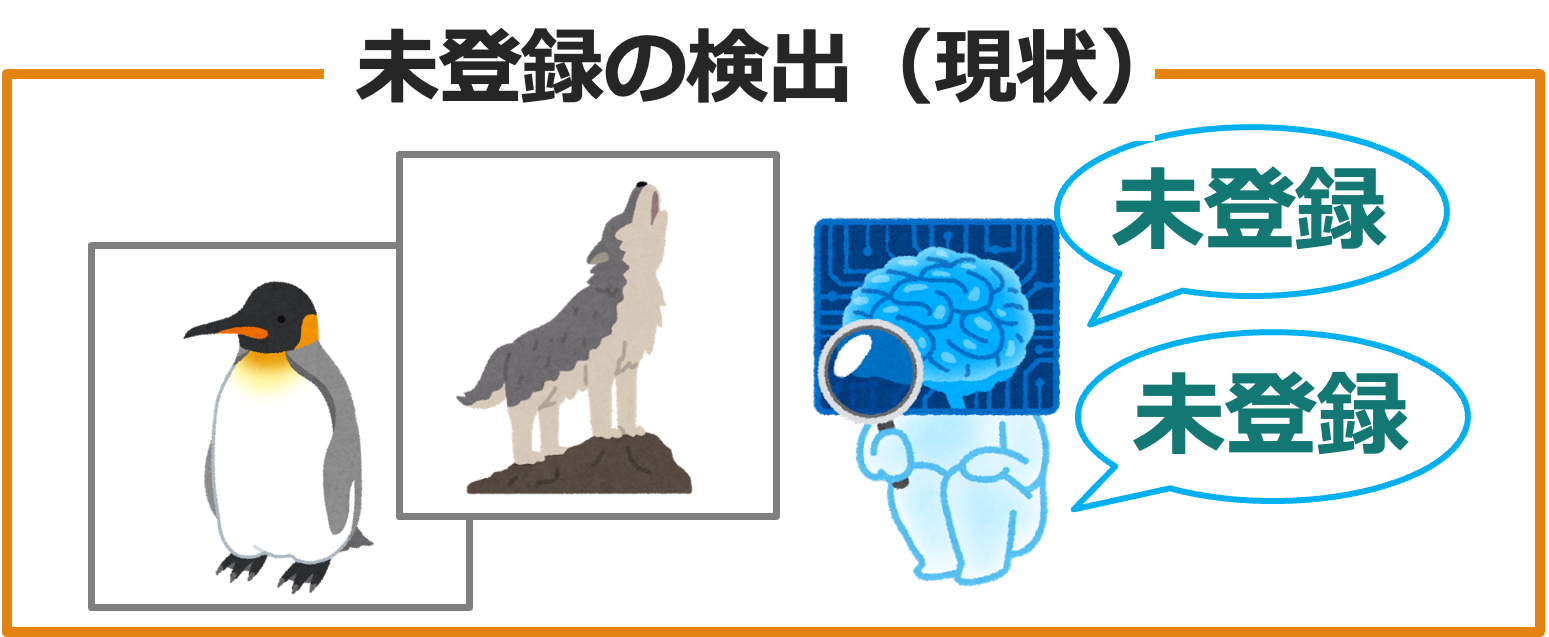
\includegraphics[width=\linewidth, keepaspectratio]{image/detection.png}
    \caption{未登録クラスの検出}
    \label{fig:detection}
  \end{subfigure}
  \hfill
  \begin{subfigure}[b]{0.45\linewidth}
    \centering
    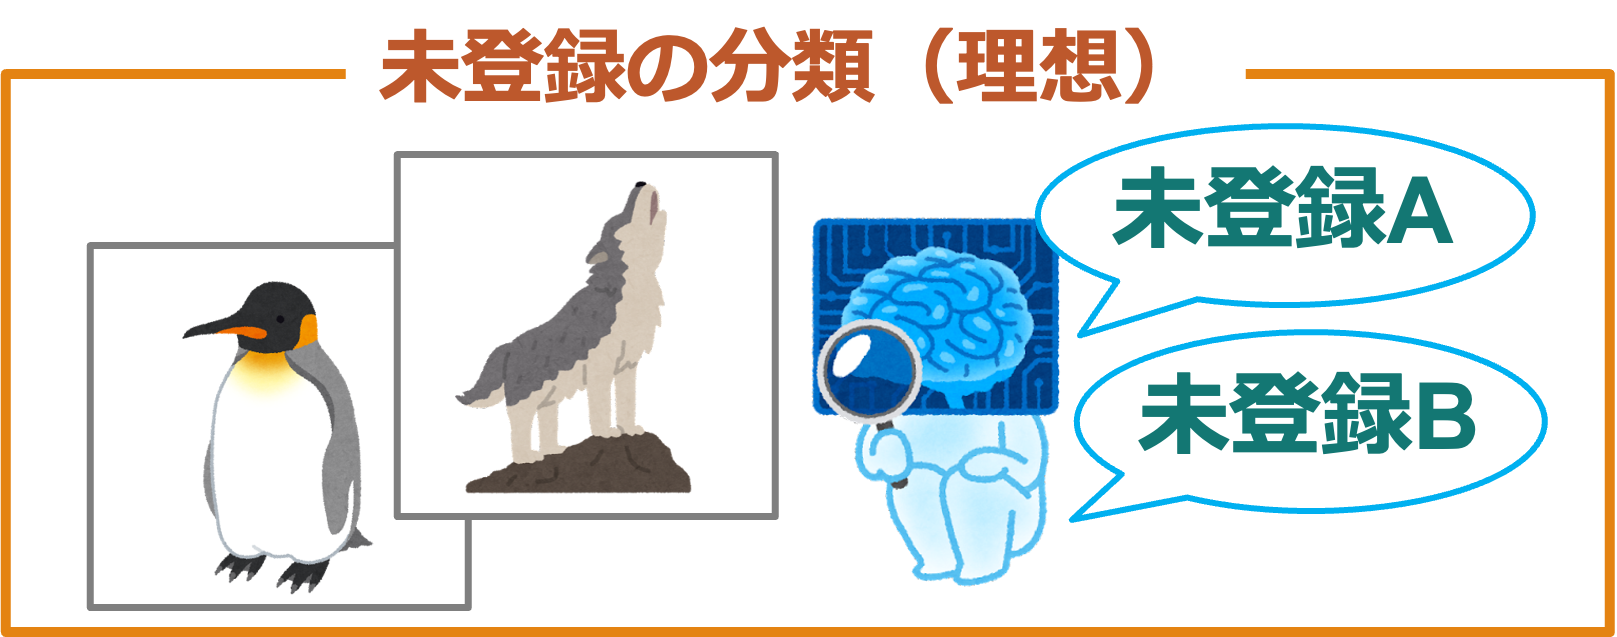
\includegraphics[width=\linewidth, keepaspectratio]{image/classification.png}
    \caption{未登録クラスの分類}
    \label{fig:classification}
  \end{subfigure}
  \caption{未登録クラスの多クラス分類}
  \label{fig:classification_goals}
\end{figure}
%
\ref{sec:detection_approach}節では,既存手法と同様に図 \ref{fig:detection}のような未登録クラスの検出に取り組んでいた.
これに対し本説ではIFORを発展させ,図 \ref{fig:classification}のような未登録クラスに対する多クラス分類精度の向上に焦点を当てている.
図 \ref{fig:feature_space}は,学習時における特徴空間上の各クラス分布を示す2つの例である.
% 
\begin{figure}[tbp]
  \centering
  \begin{subfigure}[b]{0.45\linewidth}
    \centering
    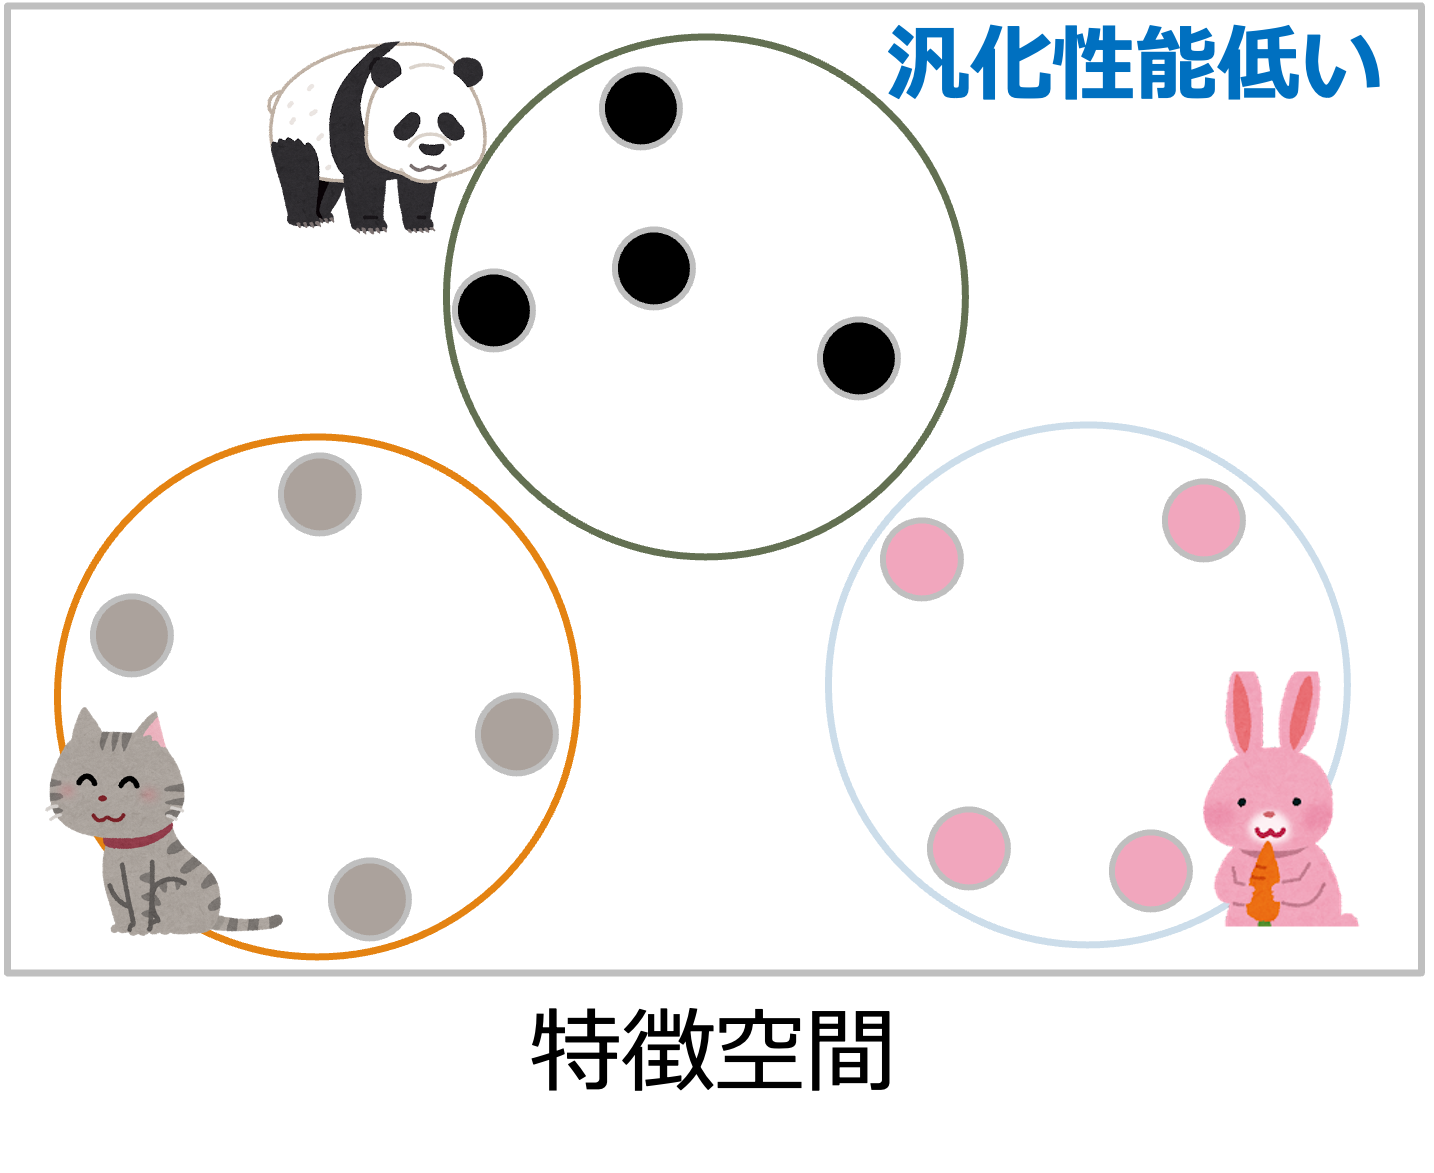
\includegraphics[height=0.9\linewidth, keepaspectratio]{image/bad_featurespace.png}
    \caption{汎化性能の低い特徴空間の例}
    \label{fig:bad_featurespace}
  \end{subfigure}
  \hfill
  \begin{subfigure}[b]{0.45\linewidth}
    \centering
    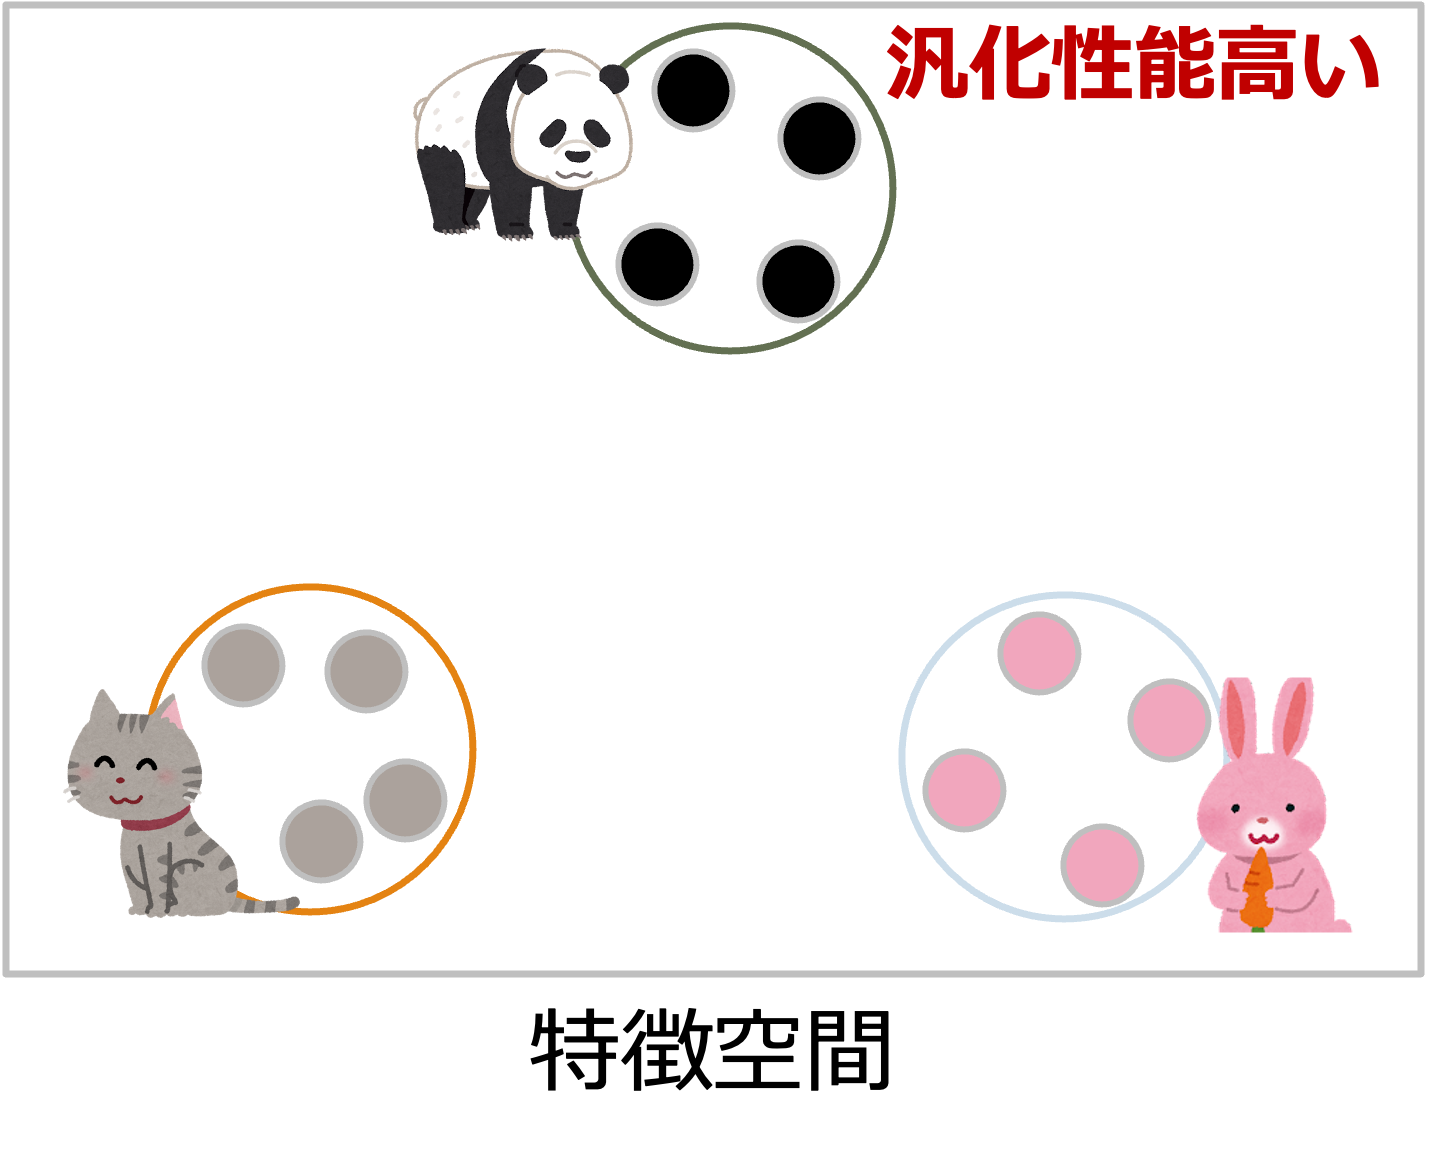
\includegraphics[height=0.9\linewidth, keepaspectratio]{image/good_featurespace.png}
    \caption{汎化性能の高い特徴空間の例}
    \label{fig:good_featurespace}
  \end{subfigure}
  \caption{学習時における特徴空間上の各クラス分布の例}
  \label{fig:feature_space}
\end{figure}
% 
四角形の枠線は特徴空間,点は特徴ベクトル,点を包含している丸い枠線はクラス分布領域の境界を表している.
図 \ref{fig:bad_featurespace}及び図 \ref{fig:good_featurespace}に示された特徴空間は,
いずれも登録済みのクラスに対して同程度の分類精度であるが,評価時のドメインシフトなどを考慮した場合,
図 \ref{fig:good_featurespace}の特徴空間の方が,新規地域に対する高い汎化性能を有していると考えられる.
これは,図 \ref{fig:good_featurespace}の方がクラス内分散が小さく,かつクラス間分散が大きいため,
新規地域においても分類が容易となるような特徴空間の構築が期待できるからである.

したがって,本研究では,メタ学習にクラスタリングに基づく損失関数を導入することにより,
クエリセットに対するクラス内分散の最小化・クラス間分散の最大化を実現する.
これにより,IFORにおける未登録クラスの多クラス化に向けて分類精度の向上を図る.

\subsection{損失関数}

本研究では,FSL損失,OSR損失,分類損失に加え,\ref{subsec:purpose}で述べたクラスタリングに基づく損失関数としてk-means損失と Between-Class損失 (BC損失)を導入する.
k-means損失は,Chinら \cite{k-means}が異常検知タスクにおいて提案した損失関数であり,k-meansクラスタリングによって集約される類似した性質を持つ特徴量から,
より識別的な特徴表現の学習を可能にする.
% より優れた特徴表現を学習するための損失関数である.
IFORフレームワークにおいて,k-means損失は以下のように定義される.

\begin{align}
\mathcal{L}_{\mathrm{k-means}} = \sum_i{\min_k \lVert f(x_i)-c_k \rVert_2}
\end{align}

\noindent
ここで,$f(x_i)$は$i$番目の入力画像を特徴抽出器$f(\cdot)$に入力した際の特徴量,$c_k$は$k$番目のクラスタ中心を表す.

k-means損失による学習の例を図 \ref{fig:kmeans_loss}に示す.
% 
\begin{figure}[tbp]
  \centering
  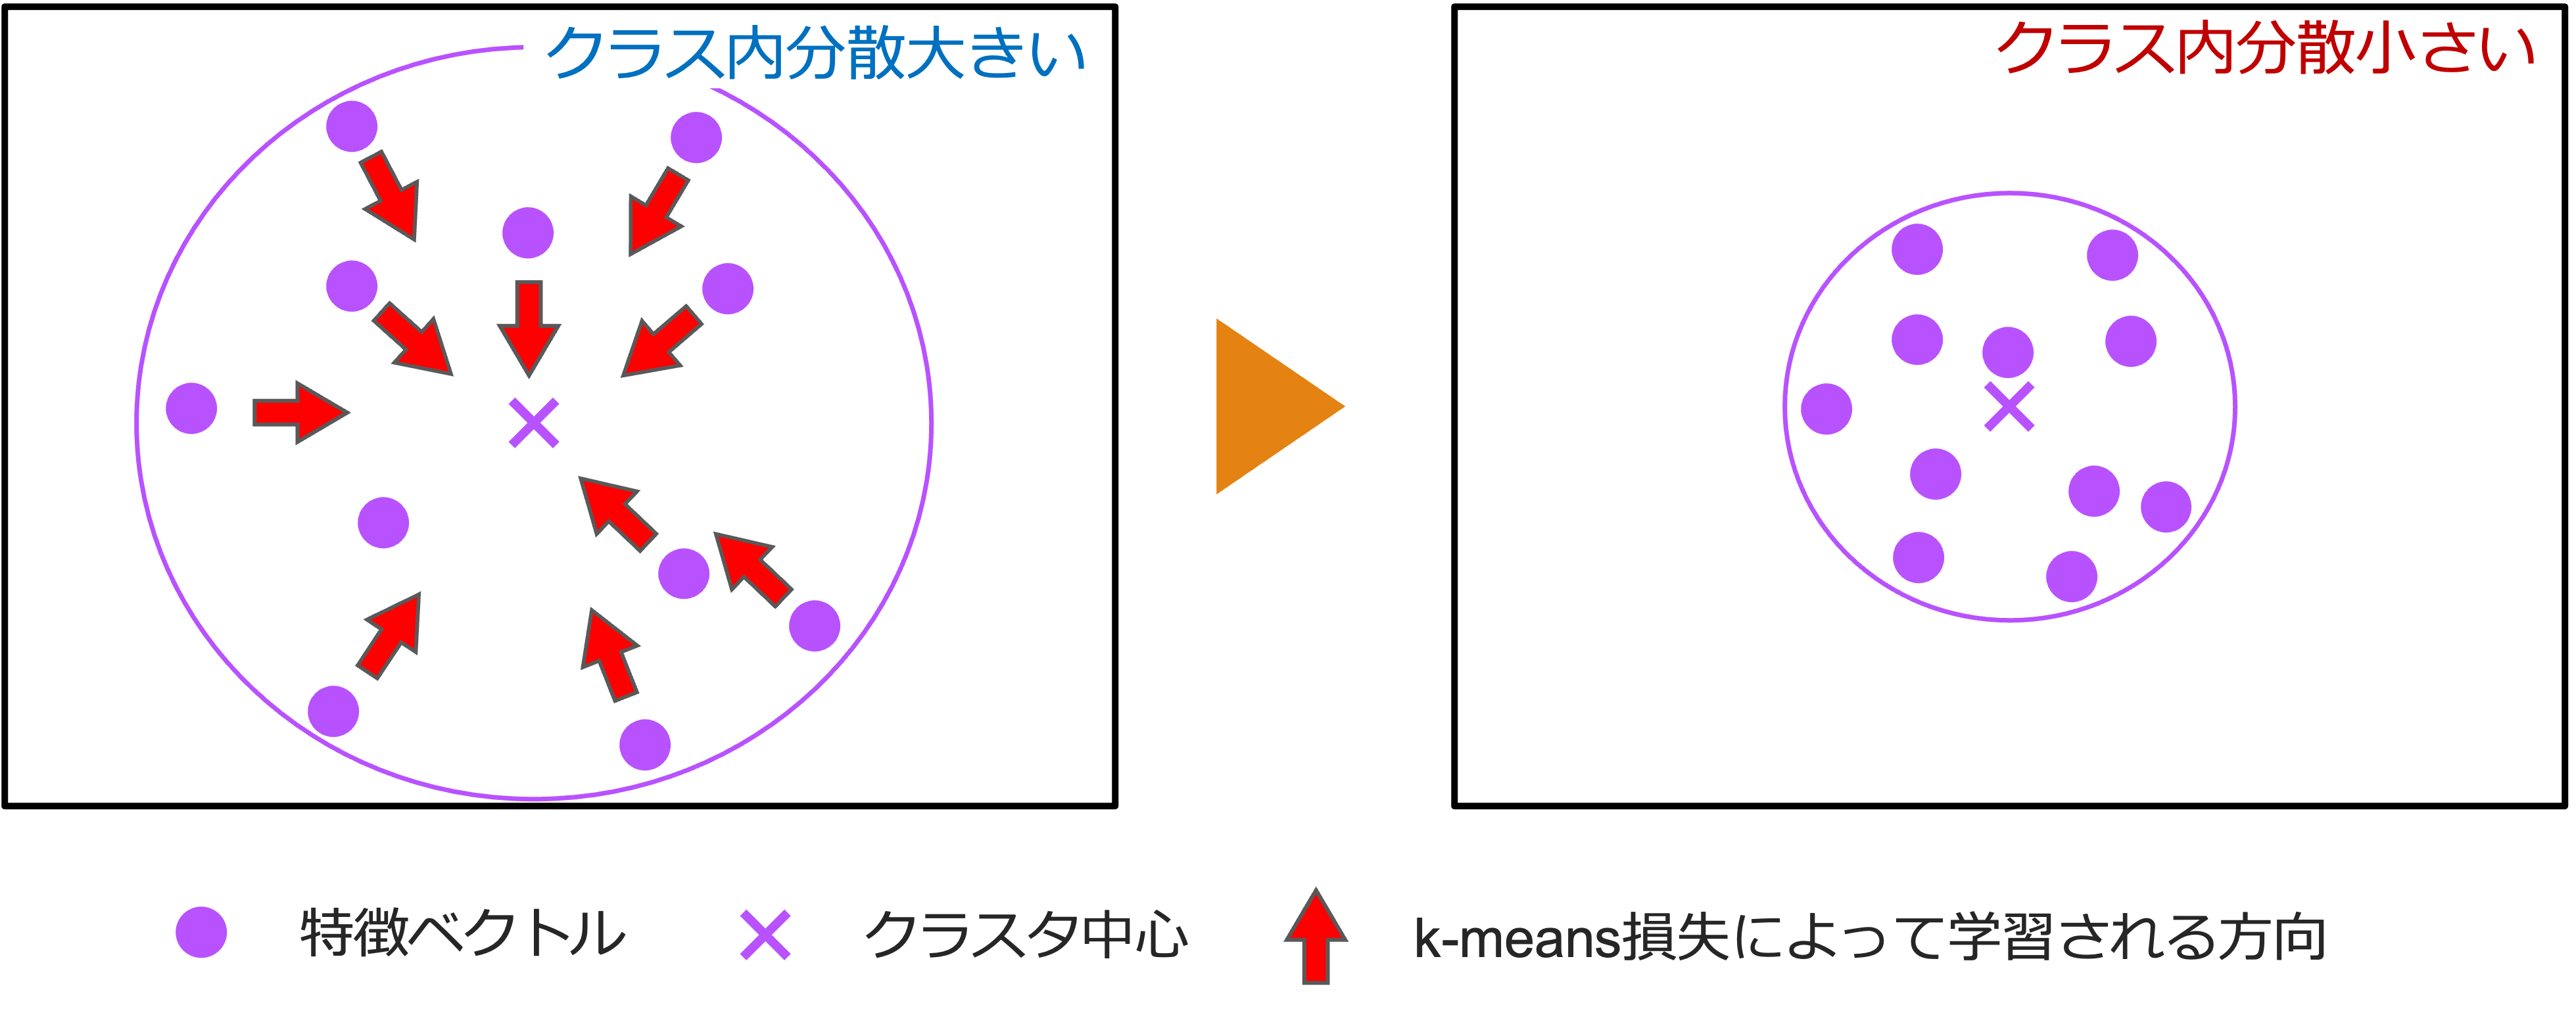
\includegraphics[width=\linewidth, keepaspectratio]{image/kmeans_loss.png}
  \caption{k-means損失によってクラス内分散が小さくなる例}
  \label{fig:kmeans_loss}
\end{figure}
% 
この損失関数の最小化により,各クラスタ中心とそのクラスタに属する特徴ベクトルとの距離が最小となることが期待される.
本研究では,類似した性質を持つ特徴量のクラスタリングにより,特徴空間上の各クラスのクラス内分散を最小化することを目指し,k-means損失の有効性を検証する.

一方,BC損失は,クラス分布のコンパクトな表現に加え,各クラスの分布が可能な限り離れているような特徴空間の構築が,
多クラス分類性能の向上に寄与するという考えに基づいている.
IFORフレームワークにおいて,BC損失は以下のように定義される.

\begin{align}
  \mathcal{L}_{\mathrm{Between-Class}} = -\log{\sum_{k_1} {\sum_{k_2} {\lVert c_{k_1} - c_{k_2} \rVert_2}}}
\end{align}

\noindent
ここで,$c_{k_1}$と$c_{k_2}$は$k_1$番目,$k_2$番目のクラスタ中心を表す.
負の符号を付与することにより,クラス間分散の最大化問題を損失関数の最小化問題として扱っている.

BC損失による学習の例を図 \ref{fig:bc_loss}に示す.
% 
\begin{figure}[tbp]
  \centering
  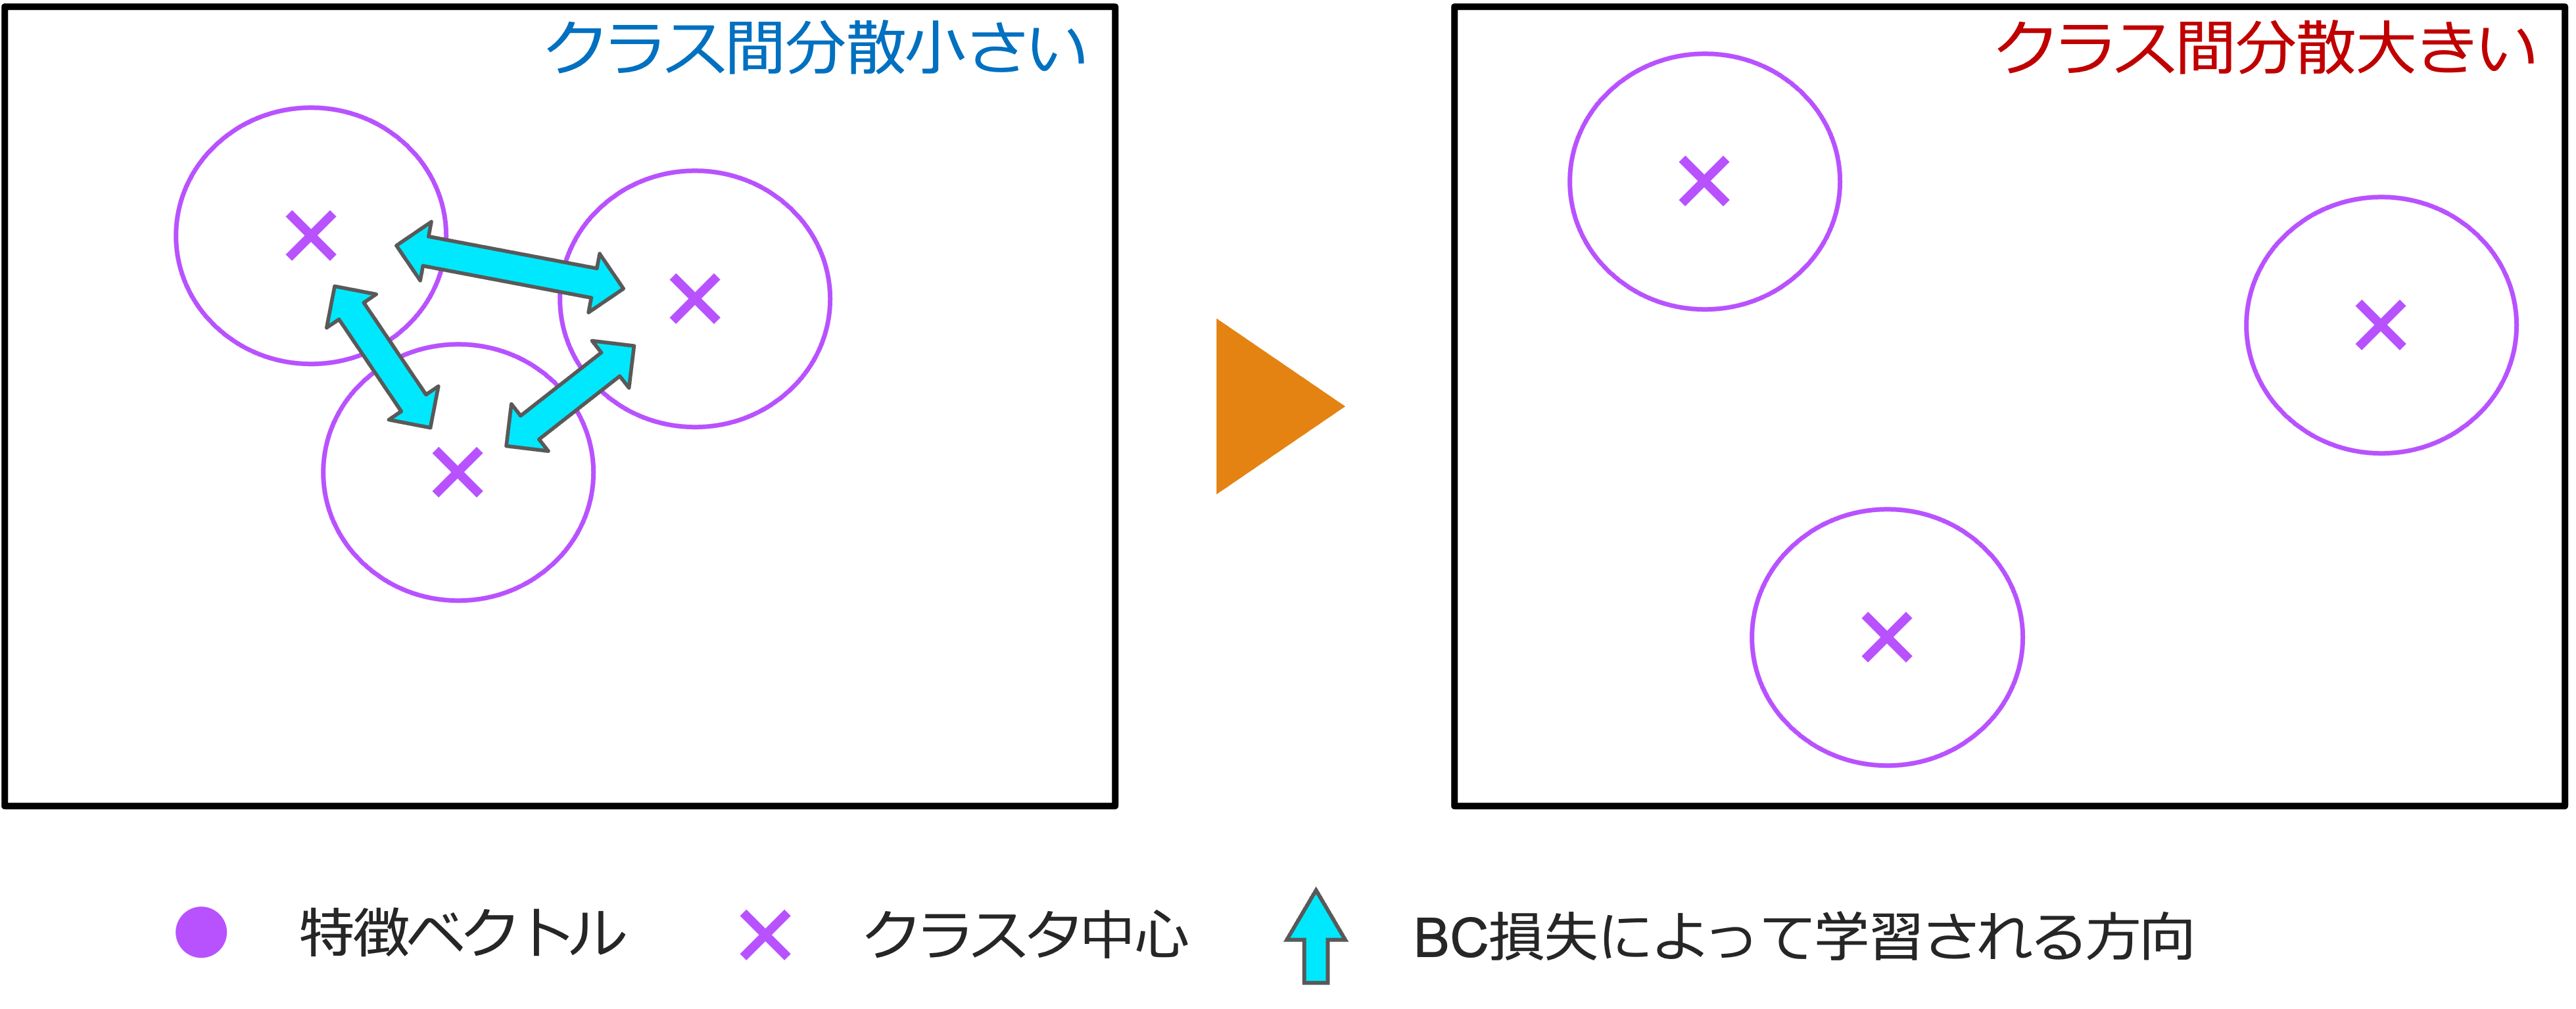
\includegraphics[width=\linewidth, keepaspectratio]{image/bc_loss.png}
  \caption{Between-Class損失によってクラス間分散が大きくなる例}
  \label{fig:bc_loss}
\end{figure}
%
この損失関数では,k-meansクラスタリングによって得られる各クラスタ中心間の距離を最大化することにより,クラス間分散の最大化を図っている.